\documentclass[12pt]{article} % Default font size is 12pt, it can be changed here

\usepackage{amsmath} %If you are writing a scientific document that contains numerous complicated formulas, the amsmath package[1] introduces several new commands that are more powerful and flexible than the ones provided by LaTeX.

\usepackage[utf8x]{inputenc}%%%%%%%%%%%%%%%%%%%%%%%%%%%%%%%%%%%%%%%%%%%%%%%%%%

\usepackage{geometry} % Required to change the page size to A4
\geometry{a4paper} % Set the page size to be A4 as opposed to the default US Letter

\usepackage{graphicx} % Required for including pictures

\usepackage{float} % Allows putting an [H] in \begin{figure} to specify the exact location of the figure
\usepackage{wrapfig} % Allows in-line images such as the example fish picture

\usepackage{lipsum} % Used for inserting dummy 'Lorem ipsum' text into the template

\usepackage{hyperref} %Used for inserting web links

\usepackage{caption}
\usepackage{subcaption}

\usepackage{nicefrac}
\usepackage{listings}
\linespread{1.15} % Line spacing

%\setlength\parindent{0pt} % Uncomment to remove all indentation from paragraphs

\graphicspath{{Pictures/}} % Specifies the directory where pictures are stored

\usepackage{booktabs}
\usepackage{amssymb}
\usepackage{longtable}
\begin{document}

%----------------------------------------------------------------------------------------
%	TITLE PAGE
%----------------------------------------------------------------------------------------

\begin{titlepage}

\newcommand{\HRule}{\rule{\linewidth}{0.5mm}} % Defines a new command for the horizontal lines, change thickness here

\center % Center everything on the page



\textsc{\LARGE Politecnico di Torino}\\[1cm] % Name of your university/college
\textsc{\Large   Bioinformatics                           }\\[0.3cm] % Major heading such as course name
%\textsc{\large                                                     }\\[0.4cm] % Minor heading such as course title

\HRule \\[0.5cm]
{ \huge  \bfseries Delegate features extraction to a Convolutional Neural Networks}\\[0.3cm] % Title of your document
\HRule \\[0.5cm]

\begin{figure}[H] % Example image
\center{
\includegraphics[width=0.5\linewidth]{Logo_Poli}}
 \end{figure}

\begin{minipage}{0.8\textwidth}
\begin{flushleft} \large
\emph{Author:}\\
Gabriele \textsc{Chiriatti}\\
 Alexander Grajales Quintero \textsc{Duverley}\\
\end{flushleft}
\end{minipage}
~
\begin{minipage}{0.4\textwidth}
\begin{flushright} \large
% Supervisor's Name
\end{flushright}
\end{minipage}\\[1.9cm]

{\large \today}\\[3cm] % Date, change the \today to a set date if you want to be precise

%\includegraphics{Logo}\\[1cm] % Include a department/university logo - this will require the graphicx package

\vfill % Fill the rest of the page with whitespace

\end{titlepage}

%----------------------------------------------------------------------------------------
%	TABLE OF CONTENTS
%----------------------------------------------------------------------------------------

\tableofcontents % Include a table of contents

\newpage % Begins the essay on a new page instead of on the same page as the table of contents 

%----------------------------------------------------------------------------------------
%	INTRODUCTION
%----------------------------------------------------------------------------------------
\begin{abstract}
We present a method to classify images with a Pre-trained Model, that are not trained for that images.
So we extract features from Pre-trained Model of Keras and after a fetures reduction, a supervised algorithm is used to classify the images. 
\end{abstract}
\newpage
%----------------------------------------------------------------------------------------
\section{Image Data Set}
The images represents histological samples of subjects looking for lung lesions. These problems can be benign or malignant.
In particular represent:
\begin{itemize}
\item Epithelioid Mesothelioma (ME)  malignant tumor.
\item Sarcomatoid Mesothelioma (MS)  malignant tumor.
\item Benign Fibrosis (F).
\end{itemize}

\begin{figure}[H] % Example image
\center{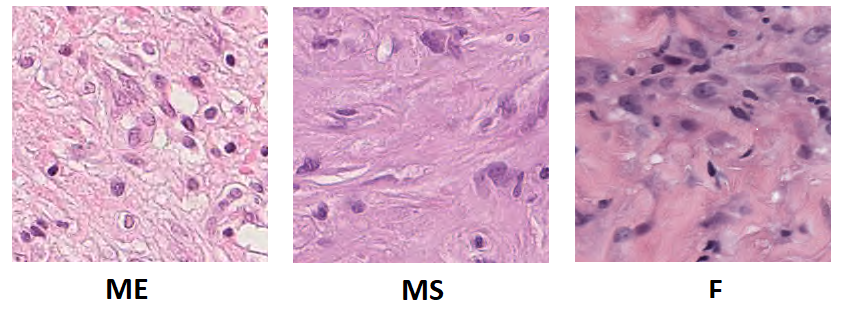
\includegraphics[width=1\linewidth]{10}}
 \end{figure}

In the Data Set there are 3104 F images, 921 ME image and 3750 MS images.

\newpage
\section{The Project}
In our work we used different Keras pre-trained model as features extractrion.\\
The model used are:
\begin{itemize}
\item VGG16
\item VGG19
\item DenseNet
\item MobileNet
\item ResNet50
\item Xception
\item NASNet
\end{itemize}

\subsection {Feature Extraction}
For our deep learning API we are using Keras which provides a high level abstraction to many of the lower level deep learning libraries like TensorFlow and Theano.
Keras as mentioned comes with a bunch of pre-trained deep learning models. These models have been trained to recognise 1000 different categories from the ImageNet database. 
However we can also use them to extract a feature vector (a list of floating point values) of the models internal representation of a category.
To get started with keras we first need to create an instance of the model we want to use.\\
The program used is called \textit{extract.py}.\\
 In this example we are using the function \textit{data\_imgnet} to select a specific model.

\begin{figure}[H] % Example image
\center{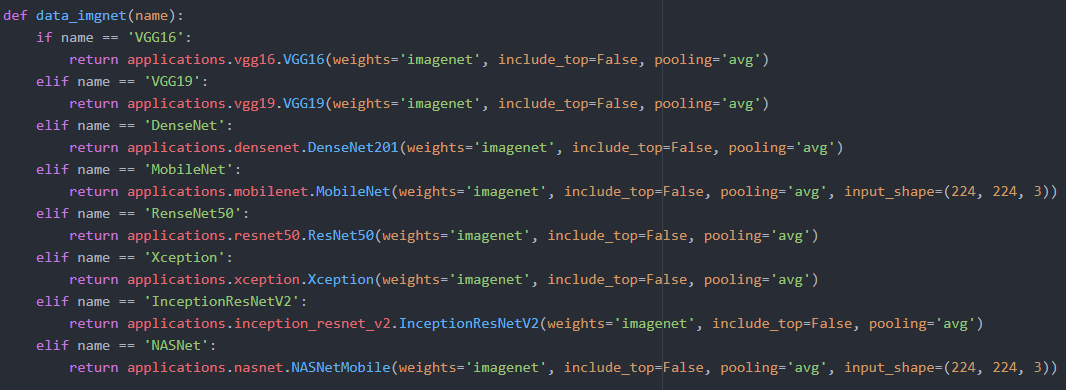
\includegraphics[width=1\linewidth]{nomi}}
 \end{figure}

Here we are setting the weights to Imagenet which will automatically download the learn parameters from the ImageNet database. The next important arg here is \textit{ include\_top=False} which removes the fully connected layer at the end/top of the network. This allows us to get the feature vector as opposed to a classification.\\
\\
Once initialised the model we can then pass it an image and use it to predict what it might be. However since we don’t want the prediction we instead will get a list of floating point values.

\begin{figure}[H] % Example image
\center{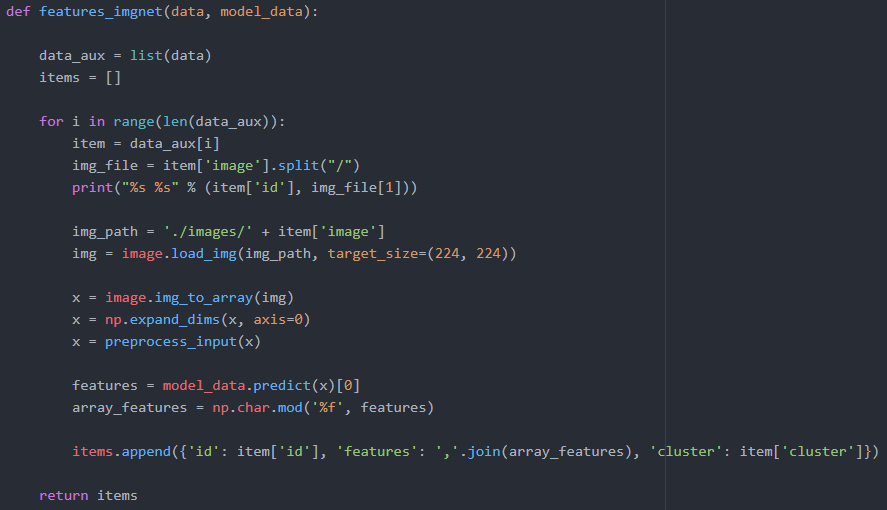
\includegraphics[width=1\linewidth]{est}}
 \end{figure}

We first load then convert our image into an array of RGB values. We then pass it into the models predict method to extract our vector.\\

\subsection {Feature Reduction}
 PCA and t-SNE  are two tools available in scikit-learn library for features reduction. In Python, scikit-learn is a widely used library for implementing machine learning algorithms. (\url{http://scikit-learn.org/stable/index.html})\\
The program used is called \textit{tecniques.py}.\\
In the function \textit{data\_model} is possible to selct (by command line) 3 different method to reduce features. Is possible to use PCA, t-SNE or a combination of both method.\\
In particular \textit{fit\_trasform (X[, y])} fit X into an embedded space and return that transformed output. 

\begin{figure}[H] % Example image
\center{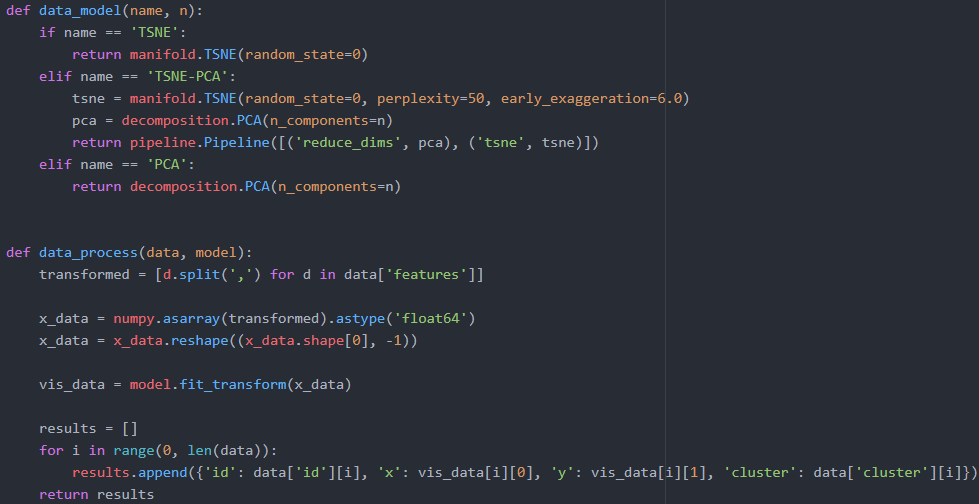
\includegraphics[width=1.10\linewidth]{model2}}
 \end{figure}

 The output of the algorithm are saved in \textit{results}:

\begin{figure}[H] % Example image
\center{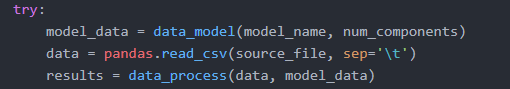
\includegraphics[width=1\linewidth]{model}}
 \end{figure}

\newpage

\subsection {Visualization of high-dimensional data in a low-dimensional space}
In order to visualize the data a reduction of our feature vector (dimensions) down to 2 is needed.\\
In our work we use three different method to do that:
\begin{itemize}
\item Use t-SNE algorithm to reduce the features down to 2.
\item Use PCA algorithm to reduce the features down to 2.
\item Use PCA and t-SNE to reduce features down to 2.
\end{itemize}
In the following example the features are extracted from the last layer in the net.\\

 \subsubsection {T-distributed Stochastic Neighbor Embedding (t-SNE)}
The image obtained for each model in this case are:\\

\begin{minipage}{0.5\textwidth}
\begin{figure}[H] % Example image
\center{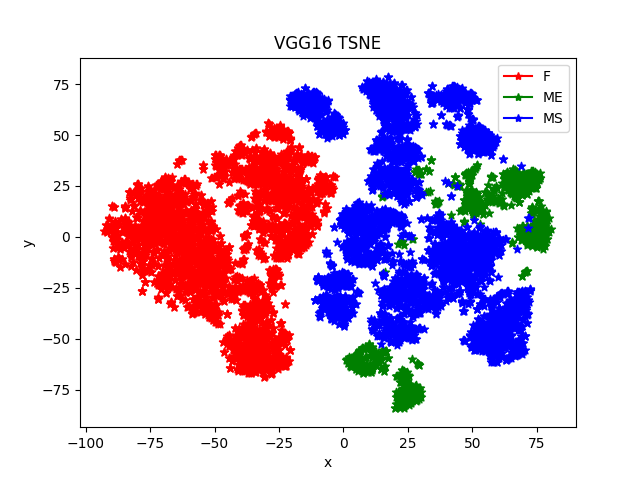
\includegraphics[width=1\linewidth]{VGG16_TSNE}}
 \end{figure}
\end{minipage}
\begin{minipage}{0.5\textwidth}
\begin{figure}[H] % Example image
\center{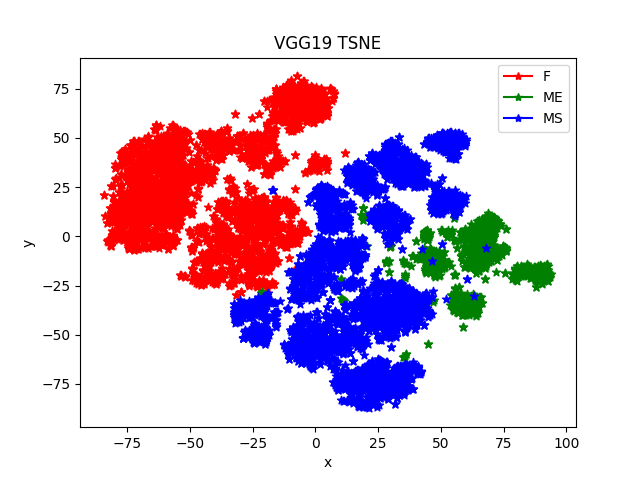
\includegraphics[width=1\linewidth]{VGG19_TSNE}}
 \end{figure}
\end{minipage}

\begin{minipage}{0.5\textwidth}
\begin{figure}[H] % Example image
\center{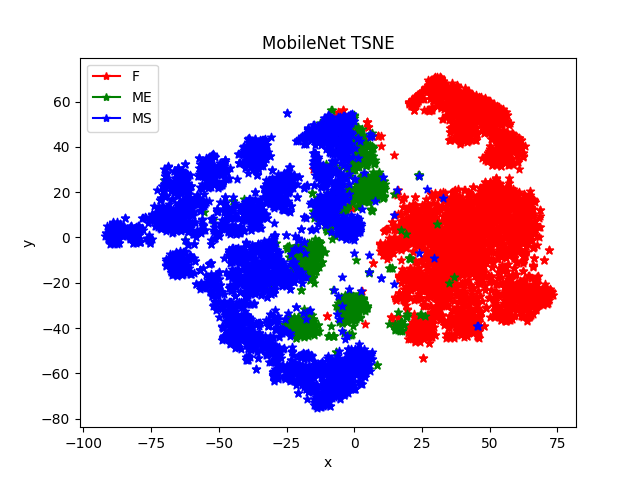
\includegraphics[width=1\linewidth]{MobileNet_TSNE}}
 \end{figure}
\end{minipage}
\begin{minipage}{0.5\textwidth}
\begin{figure}[H] % Example image
\center{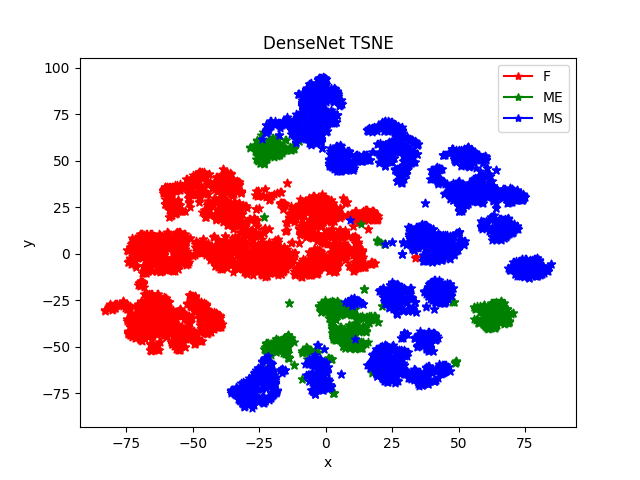
\includegraphics[width=1\linewidth]{DenseNet_TSNE}}
 \end{figure}
\end{minipage}

\begin{minipage}{0.5\textwidth}
\begin{figure}[H] % Example image
\center{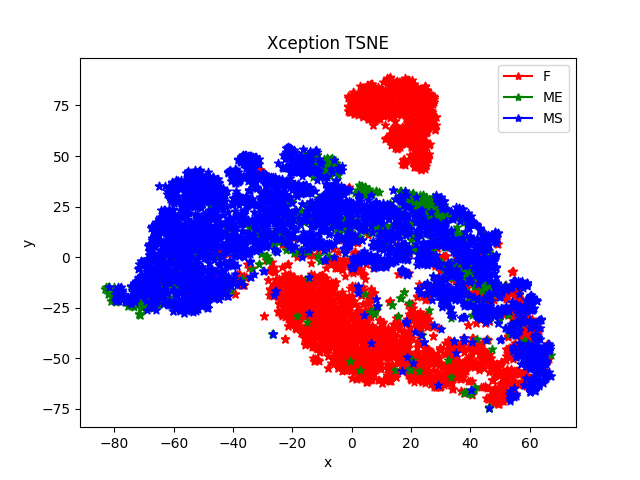
\includegraphics[width=1\linewidth]{Xception_TSNE}}
 \end{figure}
\end{minipage}
\begin{minipage}{0.5\textwidth}
\begin{figure}[H] % Example image
\center{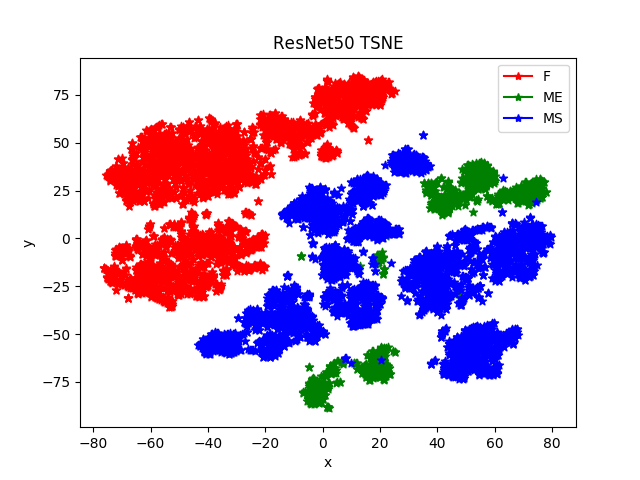
\includegraphics[width=1\linewidth]{ResNet50_TSNE}}
 \end{figure}
\end{minipage}

\begin{figure}[H] % Example image
\center{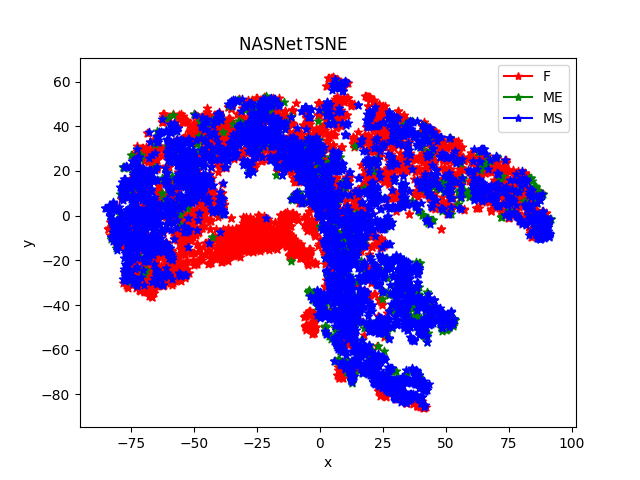
\includegraphics[width=0.5\linewidth]{NASNet_TSNE}}
 \end{figure}


 A drawback of this tecnique is that the t-SNE is not linear method so is not possible to save weights for a new image. Fine-tuning T-SNE equals tuning some heuristic-algorithm for data. This problem is not present if we use PCA.\\


\subsubsection {Principal component analysis (PCA)}
The PCA is now applicated for 2 dimensions extraction for each model\\

\begin{minipage}{0.5\textwidth}
\begin{figure}[H] % Example image
\center{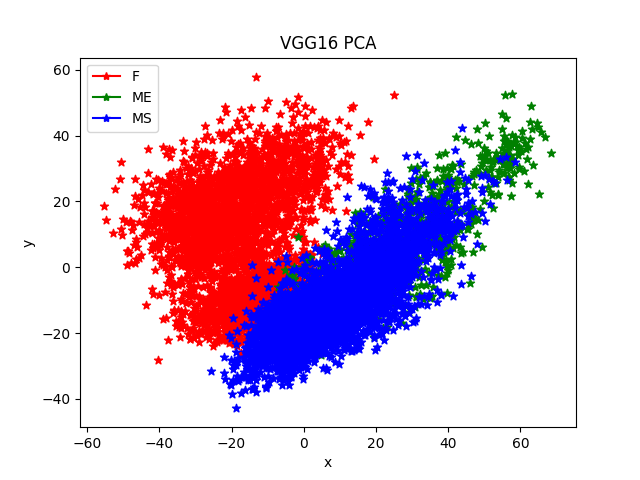
\includegraphics[width=1\linewidth]{VGG16_PCA}}
 \end{figure}
\end{minipage}
\begin{minipage}{0.5\textwidth}
\begin{figure}[H] % Example image
\center{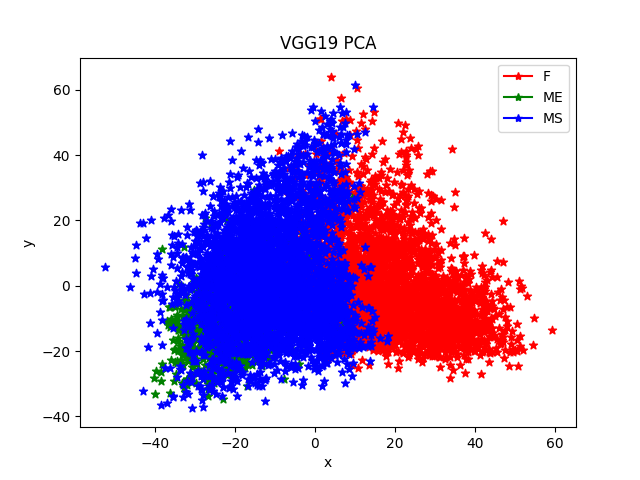
\includegraphics[width=1\linewidth]{VGG19_PCA}}
 \end{figure}
\end{minipage}

\begin{minipage}{0.5\textwidth}
\begin{figure}[H] % Example image
\center{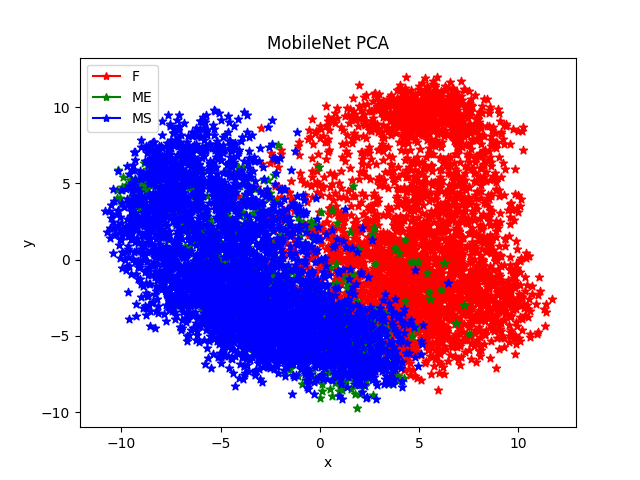
\includegraphics[width=1\linewidth]{MobileNet_PCA}}
 \end{figure}
\end{minipage}
\begin{minipage}{0.5\textwidth}
\begin{figure}[H] % Example image
\center{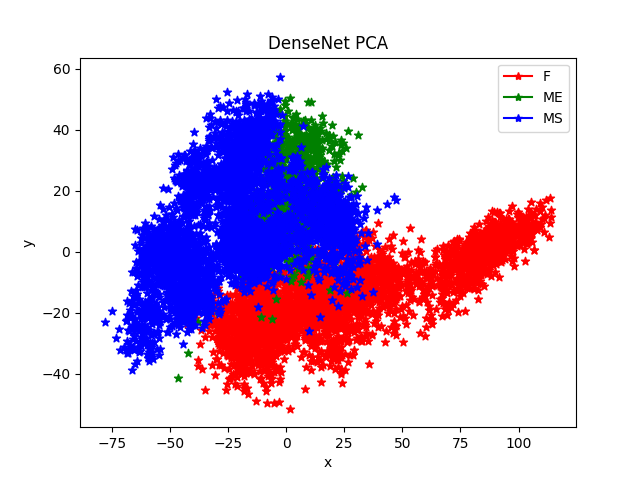
\includegraphics[width=1\linewidth]{DenseNet_PCA}}
\end{figure}
\end{minipage}

\begin{minipage}{0.5\textwidth}
\begin{figure}[H] % Example image
\center{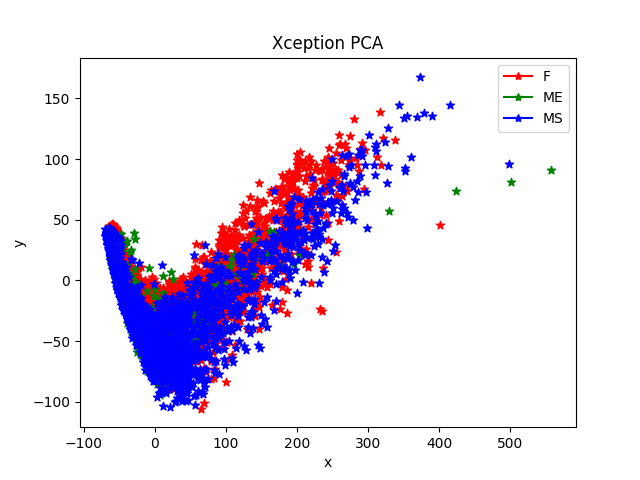
\includegraphics[width=1\linewidth]{Xception_PCA}}
 \end{figure}
\end{minipage}
\begin{minipage}{0.5\textwidth}
\begin{figure}[H] % Example image
\center{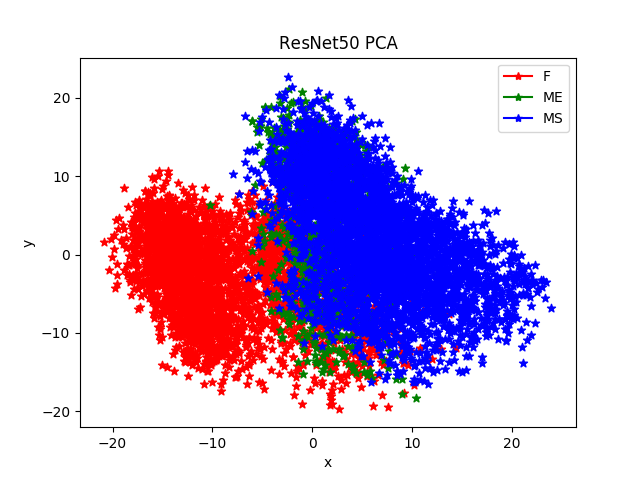
\includegraphics[width=1\linewidth]{ResNet50_PCA}}
 \end{figure}
\end{minipage}

\begin{figure}[H] % Example image
\center{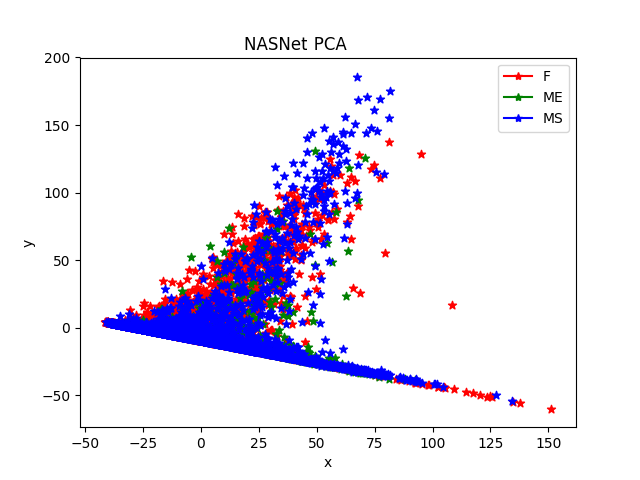
\includegraphics[width=0.5\linewidth]{NASNet_PCA}}
 \end{figure}

Is possible to see that this are the worst results. Infact is not raccomanded to use PCA to extract features down to 2. 
\subsubsection {PCA and t-SNE}
One other solution to visualize our data is to combine the two method: is possible to reduce features with PCA and use t-SNE to reduce features to two.
The optimal number of component with PCA is calculated with a funtion \textit{data\_info}. 

\begin{figure}[H] % Example image
\center{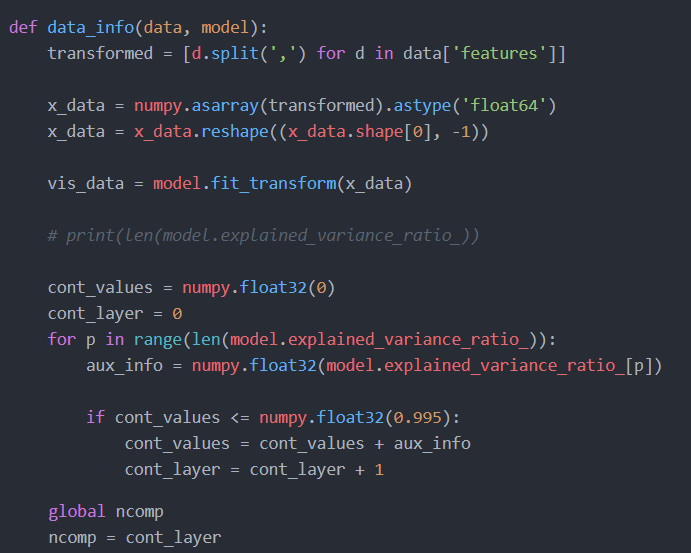
\includegraphics[width=0.7\linewidth]{func}}
\end{figure}

The command \textit{pca\_obj.explained\_variance\_ratio\_} is present in  scikit-learn library and the ouput is  a vector with percentage of variance explained by each of components. Now, we can keep adding the variance percentages until we get the desired value (in our case, 0.995). The number of required components will be the value of the variable \textit{comp}.\\ 
 The images obtained in these case are:\\

\begin{minipage}{0.5\textwidth}
\begin{figure}[H] % Example image
\center{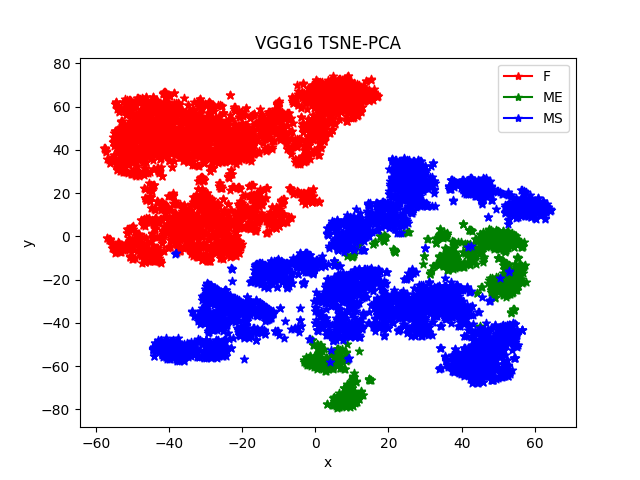
\includegraphics[width=1\linewidth]{VGG16_TSNE-PCA}}
 \end{figure}
\end{minipage}
\begin{minipage}{0.5\textwidth}
\begin{figure}[H] % Example image
\center{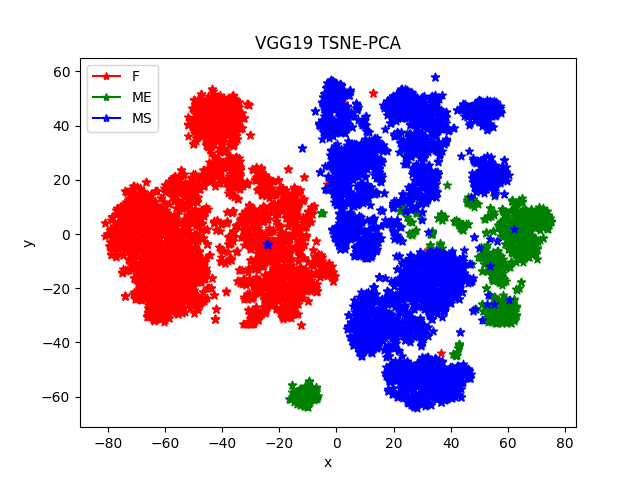
\includegraphics[width=1\linewidth]{VGG19_TSNE-PCA}}
 \end{figure}
\end{minipage}

\begin{minipage}{0.5\textwidth}
\begin{figure}[H] % Example image
\center{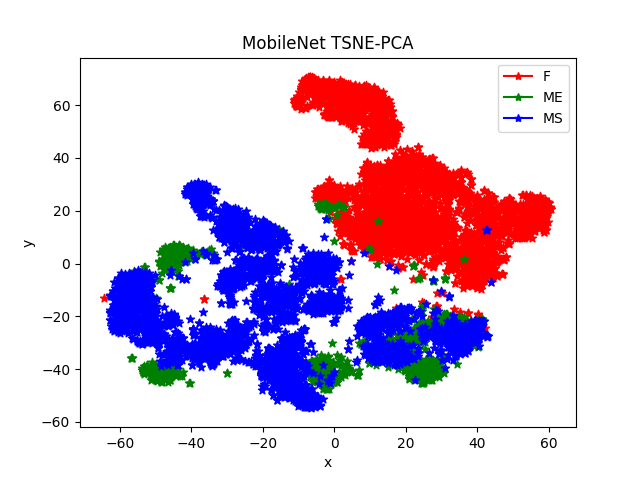
\includegraphics[width=1\linewidth]{MobileNet_TSNE-PCA}}
 \end{figure}
\end{minipage}
\begin{minipage}{0.5\textwidth}
\begin{figure}[H] % Example image
\center{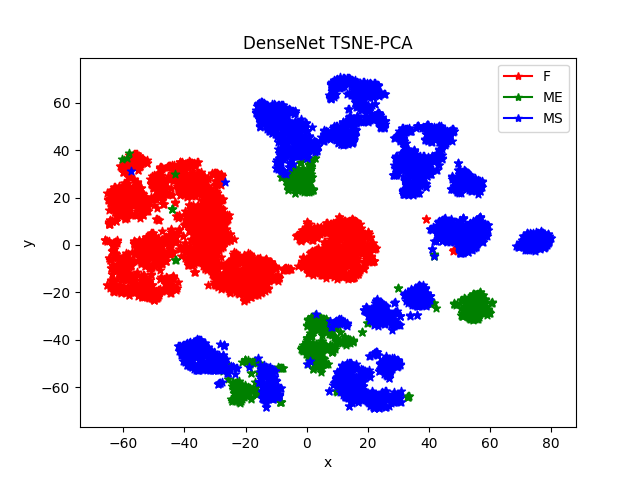
\includegraphics[width=1\linewidth]{DenseNet_TSNE-PCA}}
 \end{figure}
\end{minipage}

\begin{minipage}{0.5\textwidth}
\begin{figure}[H] % Example image
\center{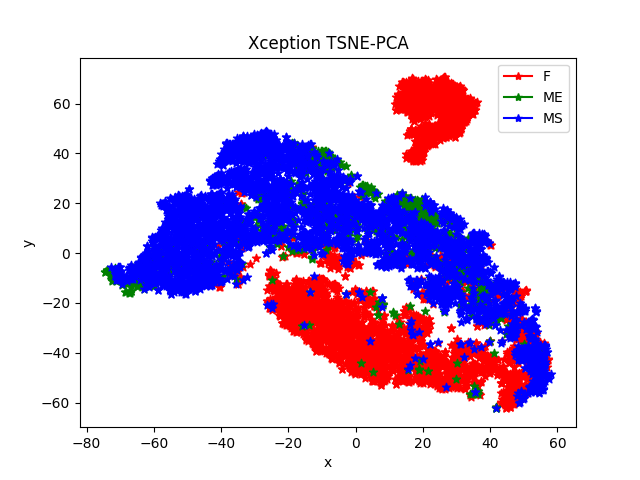
\includegraphics[width=1\linewidth]{Xception_TSNE-PCA}}
 \end{figure}
\end{minipage}
\begin{minipage}{0.5\textwidth}
\begin{figure}[H] % Example image
\center{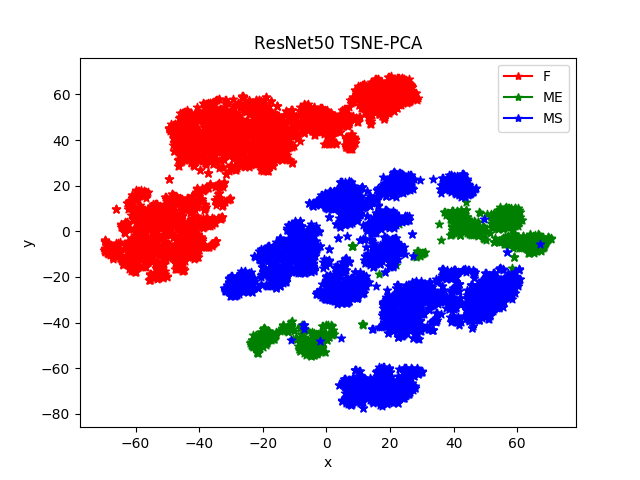
\includegraphics[width=1\linewidth]{ResNet50_TSNE-PCA}}
 \end{figure}
\end{minipage}

\begin{figure}[H] % Example image
\center{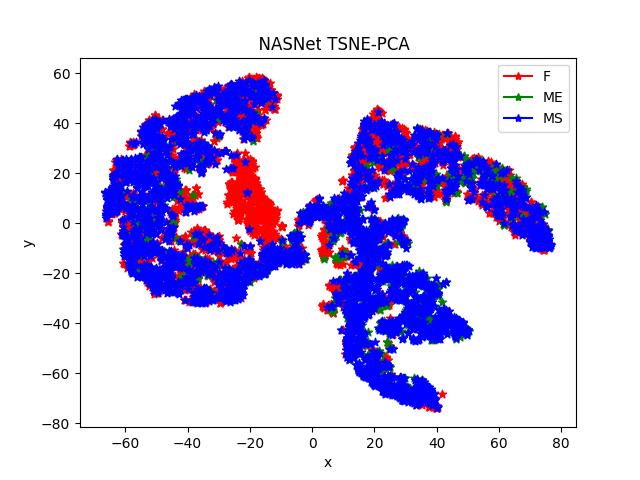
\includegraphics[width=0.5\linewidth]{NASNet_3}}
 \end{figure}

This is the best solution to visualize data infact is possible to see that the class are more defined than in the t-SNE case.

\subsection {Extract features from an arbitrary intermediate layer}
In the pre-trained model of Keras is also possible to extract features from an intermediate layer

\begin{figure}[H] % Example image
\center{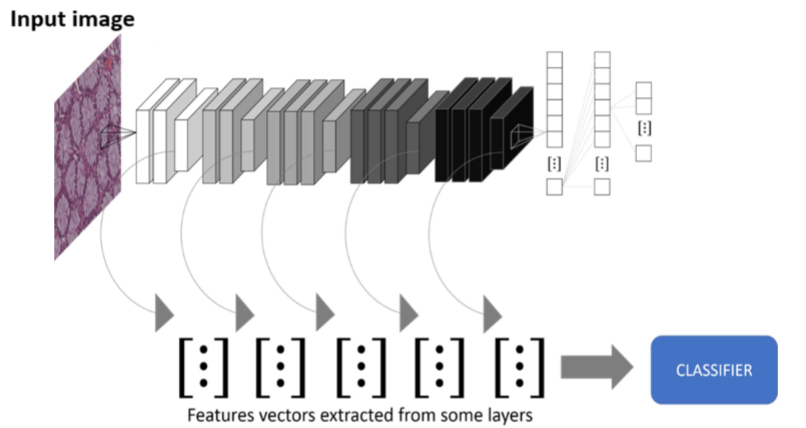
\includegraphics[width=1\linewidth]{2}}
\end{figure}

The name of the layers are visualize in the prompt during program esegution as example are reported names of VGG16 layers:

\begin{figure}[H] % Example image
\center{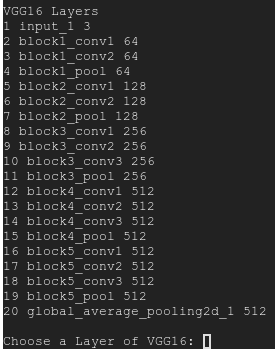
\includegraphics[width=0.3\linewidth]{image}}
\end{figure}

The user can select different output layer by number.

\begin{figure}[H] % Example image
\center{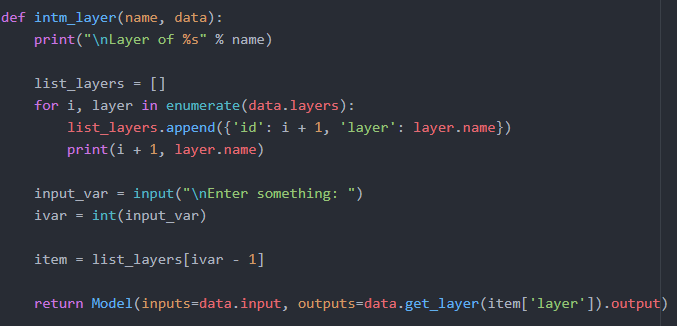
\includegraphics[width=1\linewidth]{int}}
\end{figure}

Where\textit{ layer} is the selected output layer. 

In this paper the networks was analyzed at three levels of depth:
\begin{itemize}
\item Last layer (as in previous chapter).
\item 75\%  of the net.
\item 50\%  of the net.
\item 25\%  of the net.
\end{itemize}

For each case the PCA and t-SNE algorithm are applicated in order to visualize the data in 2D.\\

\subsubsection {75\%  of the net}
The images obtained with PCA and t-SNE for each model are:\\

\begin{minipage}{0.5\textwidth}
\begin{figure}[H] % Example image
\center{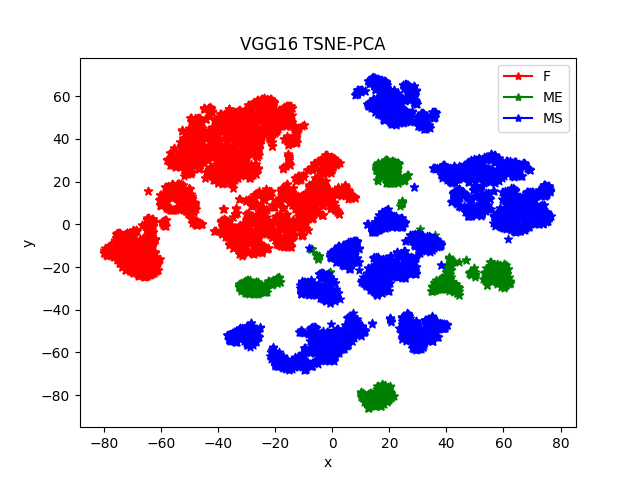
\includegraphics[width=1\linewidth]{VGG16_75}}
 \end{figure}
\end{minipage}
\begin{minipage}{0.5\textwidth}
\begin{figure}[H] % Example image
\center{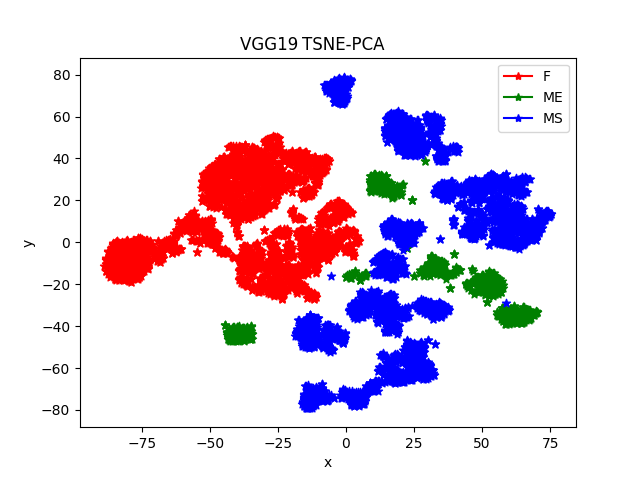
\includegraphics[width=1\linewidth]{VGG19_75}}
 \end{figure}
\end{minipage}

\begin{minipage}{0.5\textwidth}
\begin{figure}[H] % Example image
\center{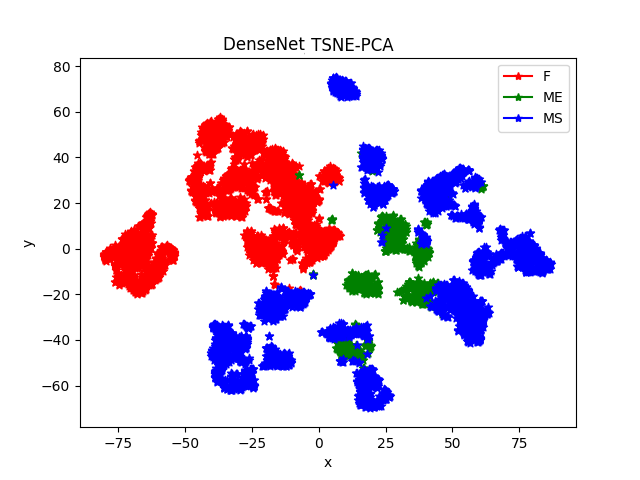
\includegraphics[width=1\linewidth]{DenseNet_75}}
 \end{figure}
\end{minipage}
\begin{minipage}{0.5\textwidth}
\begin{figure}[H] % Example image
\center{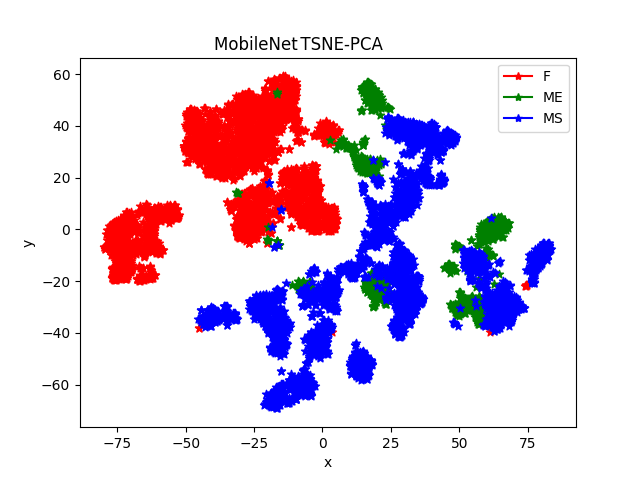
\includegraphics[width=1\linewidth]{MobileNet_75}}
 \end{figure}
\end{minipage}

\begin{minipage}{0.5\textwidth}
\begin{figure}[H] % Example image
\center{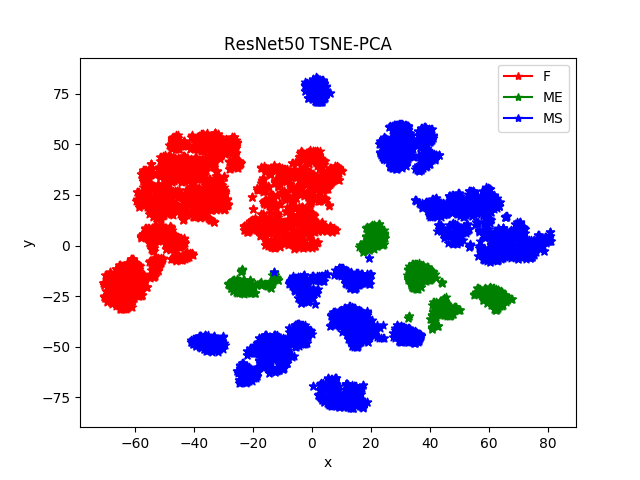
\includegraphics[width=1\linewidth]{ResNet50_75}}
 \end{figure}
\end{minipage}
\begin{minipage}{0.5\textwidth}
\begin{figure}[H] % Example image
\center{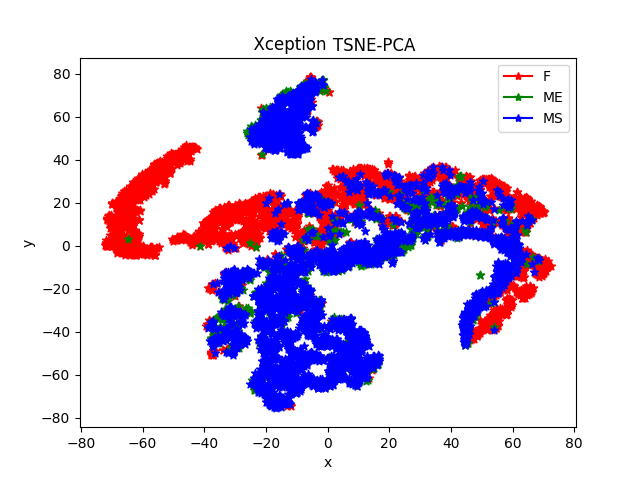
\includegraphics[width=1\linewidth]{Xception_75}}
 \end{figure}
\end{minipage}

\begin{figure}[H] % Example image
\center{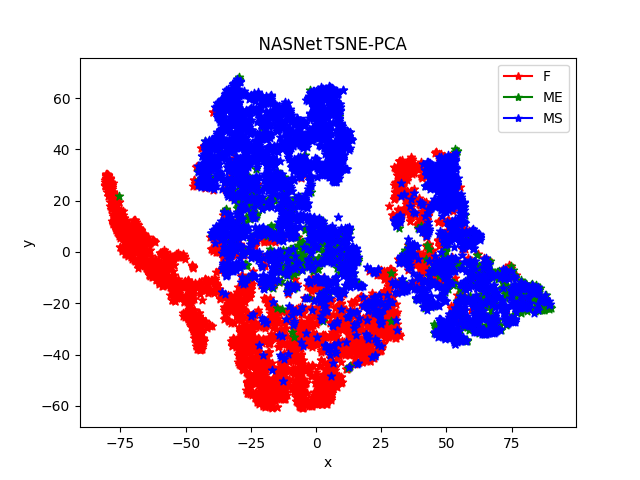
\includegraphics[width=0.5\linewidth]{NASNet_75}}
 \end{figure}

\subsubsection {50\%  of the net}
The images obtained with PCA and t-SNE for each model are:\\

\begin{minipage}{0.5\textwidth}
\begin{figure}[H] % Example image
\center{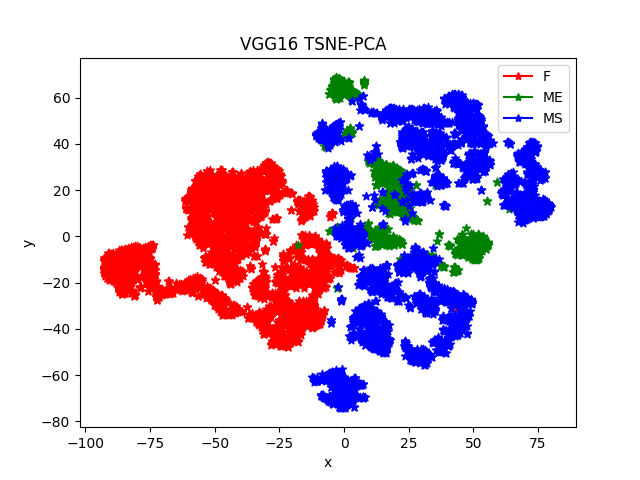
\includegraphics[width=1\linewidth]{VGG16_50}}
 \end{figure}
\end{minipage}
\begin{minipage}{0.5\textwidth}
\begin{figure}[H] % Example image
\center{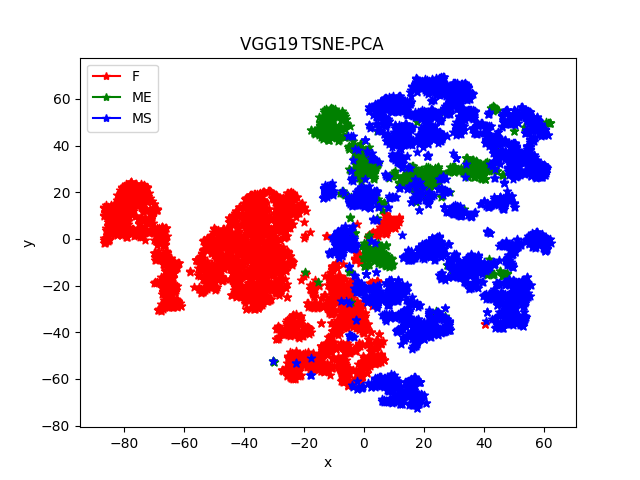
\includegraphics[width=1\linewidth]{VGG19_50}}
 \end{figure}
\end{minipage}

\begin{minipage}{0.5\textwidth}
\begin{figure}[H] % Example image
\center{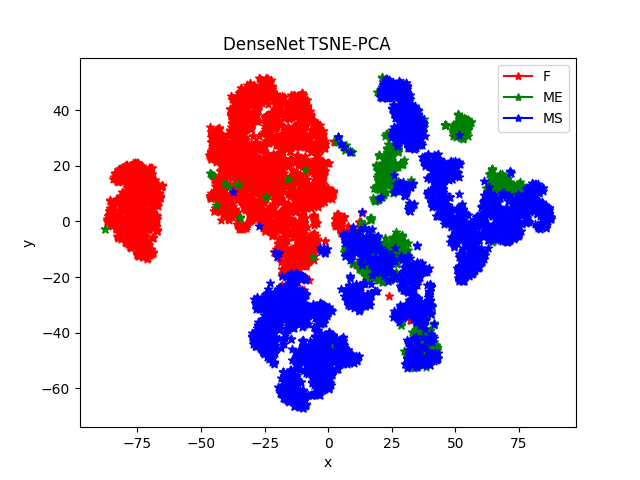
\includegraphics[width=1\linewidth]{DenseNet_50}}
 \end{figure}
\end{minipage}
\begin{minipage}{0.5\textwidth}
\begin{figure}[H] % Example image
\center{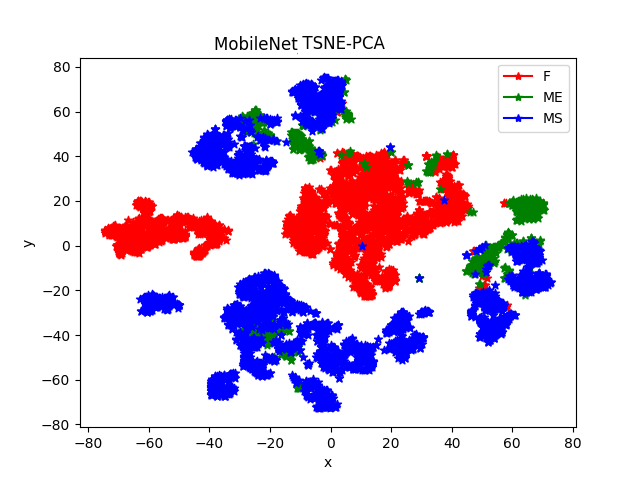
\includegraphics[width=1\linewidth]{MobileNet_50}}
 \end{figure}
\end{minipage}

\begin{minipage}{0.5\textwidth}
\begin{figure}[H] % Example image
\center{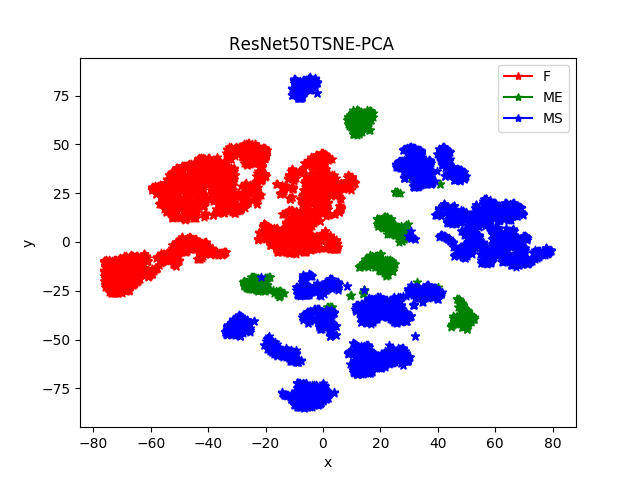
\includegraphics[width=1\linewidth]{ResNet50_50}}
 \end{figure}
\end{minipage}
\begin{minipage}{0.5\textwidth}
\begin{figure}[H] % Example image
\center{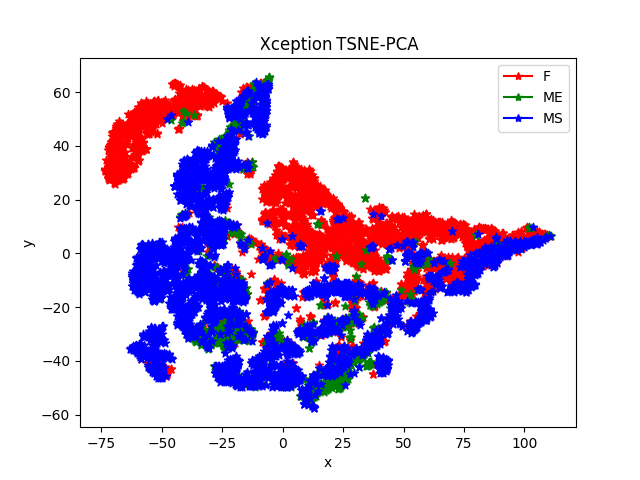
\includegraphics[width=1\linewidth]{Xception_50}}
 \end{figure}
\end{minipage}

\begin{figure}[H] % Example image
\center{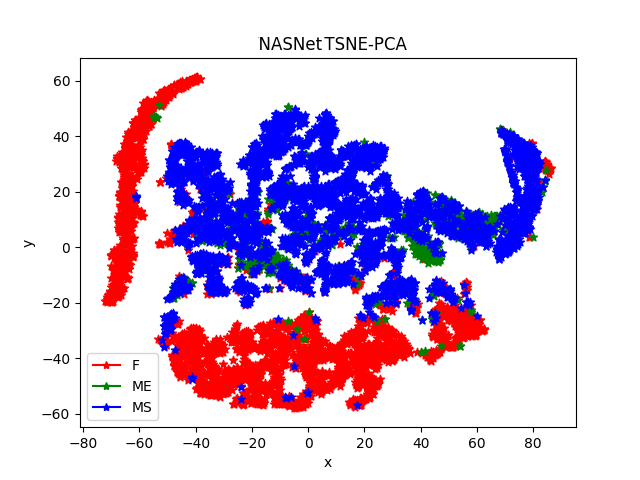
\includegraphics[width=0.5\linewidth]{NASNet_50}}
 \end{figure}

\subsubsection {25\%  of the net}
The images obtained with PCA and t-SNE for each model are:\\

\begin{minipage}{0.5\textwidth}
\begin{figure}[H] % Example image
\center{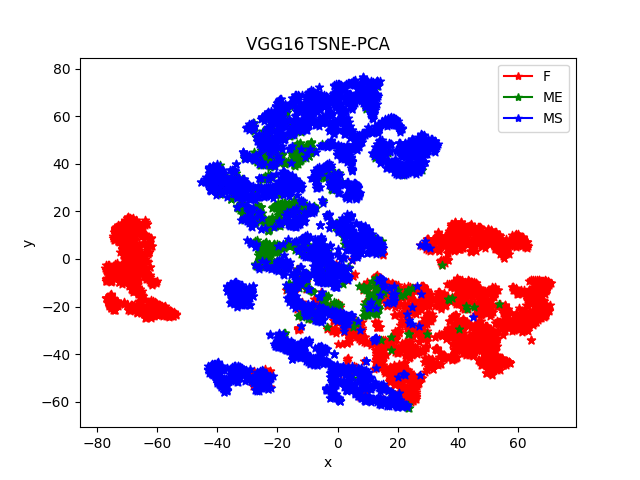
\includegraphics[width=1\linewidth]{VGG16_25}}
 \end{figure}
\end{minipage}
\begin{minipage}{0.5\textwidth}
\begin{figure}[H] % Example image
\center{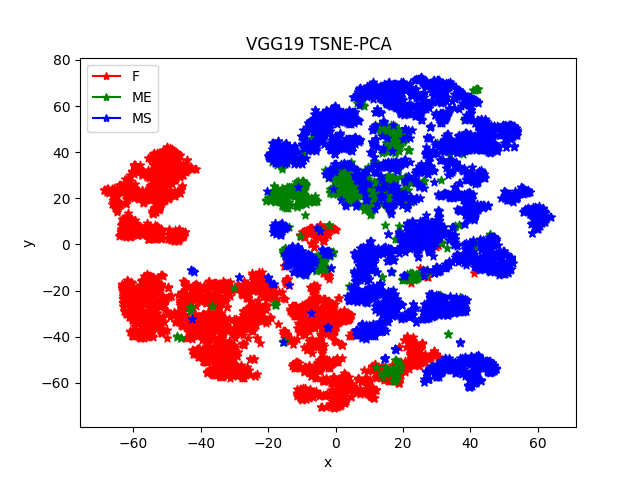
\includegraphics[width=1\linewidth]{VGG19_25}}
 \end{figure}
\end{minipage}

\begin{minipage}{0.5\textwidth}
\begin{figure}[H] % Example image
\center{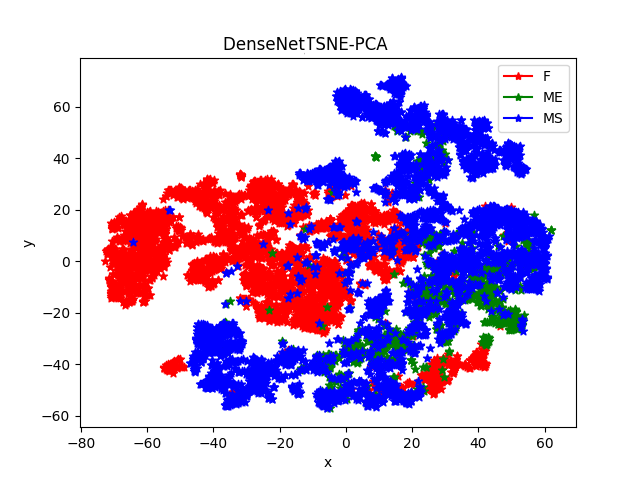
\includegraphics[width=1\linewidth]{DenseNet_25}}
 \end{figure}
\end{minipage}
\begin{minipage}{0.5\textwidth}
\begin{figure}[H] % Example image
\center{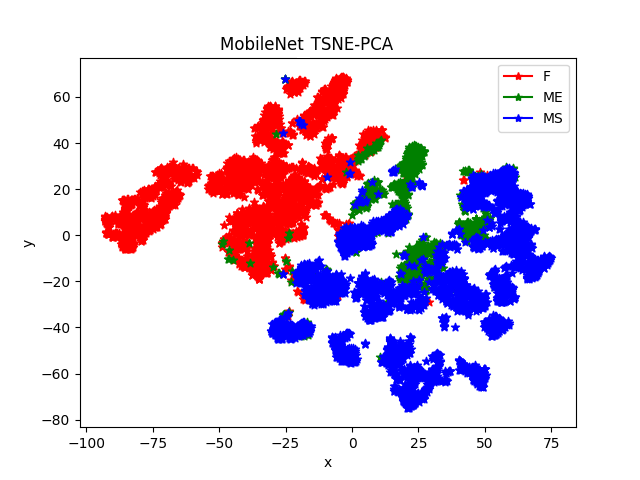
\includegraphics[width=1\linewidth]{MobileNet_25}}
 \end{figure}
\end{minipage}

\begin{minipage}{0.5\textwidth}
\begin{figure}[H] % Example image
\center{\includegraphics[width=1\linewidth]{ResNet50_25}}
 \end{figure}
\end{minipage}
\begin{minipage}{0.5\textwidth}
\begin{figure}[H] % Example image
\center{\includegraphics[width=1\linewidth]{Xception_25}}
 \end{figure}
\end{minipage}

\begin{figure}[H] % Example image
\center{\includegraphics[width=0.5\linewidth]{NASNet_25}}
 \end{figure}
%%%%%%%%%%%%%%%%%%%%%%%%%%%%%%%%%%%%%%%%%%%%%%%%%%%%%%%%%%%%%%%%%%%%%%%%%%%%%%%%%%
\newpage

\subsection {Supervised Classifier}
In order to classify our image a Supervised Classifier is needed.\\
In our work we used two different classifier:

\begin{itemize}
\item k-NN:k-nearest neighbors.
\item SVM:Support Vector Machine.
\end{itemize}

\subsubsection {k-NN}
The Classifier is based on k-NN method and use the Euclidian distance from points.
The program used is called \textit{KNN.py}.\\
\begin{figure}[H] % Example image
\center{\includegraphics[width=0.8\linewidth]{knn}}
\end{figure}
In particular the function \textit{dist\_euclidian} computes the distance. The function \textit{get\_nbr} select the neighbour of the new test point. The number of neighbour is selected by the user. \\
The classifier is able to predict the label of the test point based to his neighbour. \\
The training set is chosen randomically. The training and test set are made with the function \textit{load\_dataset}.
\begin{figure}[H] % Example image
\center{\includegraphics[width=0.8\linewidth]{datas}}
\end{figure}
In our code \textit{num\_split} is the percentage of elements used as training set and it can be modify by user. The used value is 0.7. (70\% for training set)
The other elements are used as test set and a confusion matrix is obtained in order to calculate the average accuracy of the model.\\  

The choice of the number of neighbors (k) is made according these rules:
\begin{itemize}
\item  k value should be odd.
\item  k value must not be multiples of the number of classes.
\item  Should not be too small or too large
\end{itemize}
An empiric formula to calculate it is to use $sqrt(n)$ where n is the size of the training data (reference \url{https://arxiv.org/ftp/arxiv/papers/1409/1409.0919.pdf}) but in our case the number is too large (25 neighbors).\\
For the computational cost of k-NN a small number of neighbour is needed.\\
We decide to use 5 neighbors because respect the rules and the computational cost is not so large. 

\subsubsection {SVM}
SVM  is available in scikit-learn library and follow the structure:Import library, object creation, fitting model and prediction. 
Is possible to use the library to call SVC method  for multiclass classification.
The program used is called \textit{SVM.py}.\\
The method analysed are:
\begin{itemize}
\item  \textit{"ovo":one-vs-one}.
\item  \textit{"ovr":one-vs-rest}.
\end{itemize}
With the function  \textit{name\_svm} is possible to select the method.
\begin{figure}[H] % Example image
\center{\includegraphics[width=1\linewidth]{svm}}
\end{figure}
After that is possible to train the model and to test it. The test/training set is chosen, as in previous case, with the function \textit{load\_dataset}.

\newpage 

\subsection {Results}
The accuracy of both classifiers are also based on PCA reduction. The number of component of the features, after PCA reduction is chosen by the user.
In our work we used the function\textit{data\_info},as mentioned, to try to calculate the optimal number of component for PCA.\\

\begin{center}
\begin{tabular}{l|c|c|c|c|}
 \multicolumn{5}{c}{ \textbf{ PCA optimal number component}}\\
 \textbf{Depth}&25\%&50\%&75\%&Last layer\\ \hline\hline
VGG16   &10&81&355&304\\
VGG19 &24&29&342&301\\
MobileNet &17&51&157&539\\
DenseNet &19&22&16&249\\
ResNet50 &49&56&628&940\\
Xception&18&32&31&262\\
\end{tabular}
\end{center}

\subsubsection {k-NN}
The result of k-NN classifier are reported through a confusion matrix for each pre trained model.\\
The output are calculted for k=5.\\
\begin{center}
\textbf{ VGG16 k=5}
\end{center}
\begin{minipage}{0.5\textwidth}
\begin{center}
\begin{tabular}{l|c|c|c|}
 \multicolumn{4}{c}{ \textbf{ Predicted}}\\
 \textbf{Know}&F&ME&MS\\ \hline\hline
F   &0.999&0&0.001\\
ME &0&0.99&0.001\\
MS &0&0.005&0.995\\
\multicolumn{4}{c}{Average Accuracy is 0.99}\\
\multicolumn{4}{c}{Last layer}\\
\end{tabular}
\end{center}
\end{minipage}
\begin{minipage}{0.5\textwidth}
\begin{center}
\begin{tabular}{l|c|c|c|}
 \multicolumn{4}{c}{ \textbf{ Predicted}}\\
 \textbf{Know}&F&ME&MS\\ \hline\hline
F   &1&0&0\\
ME &0&1&0\\
MS &0&0.002&0.0.998\\
\multicolumn{4}{c}{Average Accuracy is 0.99}\\
\multicolumn{4}{c}{75\%  of the net}\\
\end{tabular}
\end{center}
\end{minipage}
\begin{minipage}{0.5\textwidth}
\begin{center}
\begin{tabular}{l|c|c|c|}
 \multicolumn{4}{c}{ \textbf{ Predicted}}\\
 \textbf{Know}&F&ME&MS\\ \hline\hline
F   &1&0&0\\
ME &0&0.993&0.007\\
MS &0&0.0004&0.996\\
\multicolumn{4}{c}{Average Accuracy is 0.99}\\
\multicolumn{4}{c}{50\%  of the net}\\
\end{tabular}
\end{center}
\end{minipage}
\begin{minipage}{0.5\textwidth}
\begin{center}
\begin{tabular}{l|c|c|c|}
 \multicolumn{4}{c}{ \textbf{ Predicted}}\\
 \textbf{Know}&F&ME&MS\\ \hline\hline
F   &0.994&0&0.006\\
ME &0.01&0.85&0.14\\
MS &0&0.01&0.99\\
\multicolumn{4}{c}{Average Accuracy is 0.94}\\
\multicolumn{4}{c}{25\%  of the net}\\
\end{tabular}
\end{center}
\end{minipage}

\begin{center}
\textbf{ VGG19 k=5}
\end{center}
\begin{minipage}{0.5\textwidth}
\begin{center}
\begin{tabular}{l|c|c|c|}
 \multicolumn{4}{c}{ \textbf{ Predicted}}\\
 \textbf{Know}&F&ME&MS\\ \hline\hline
F   &0.999&0&0.001\\
ME &0&0.99&0.001\\
MS &0&0.005&0.995\\
\multicolumn{4}{c}{Average Accuracy is 0.99}\\
\multicolumn{4}{c}{Last layer}\\
\end{tabular}
\end{center}
\end{minipage}
\begin{minipage}{0.5\textwidth}
\begin{center}
\begin{tabular}{l|c|c|c|}
 \multicolumn{4}{c}{ \textbf{ Predicted}}\\
 \textbf{Know}&F&ME&MS\\ \hline\hline
F   &1&0&0\\
ME &0&1&0\\
MS &0&0.002&0.0.998\\
\multicolumn{4}{c}{Average Accuracy is 0.99}\\
\multicolumn{4}{c}{75\%  of the net}\\
\end{tabular}
\end{center}
\end{minipage}
\begin{minipage}{0.5\textwidth}
\begin{center}
\begin{tabular}{l|c|c|c|}
 \multicolumn{4}{c}{ \textbf{ Predicted}}\\
 \textbf{Know}&F&ME&MS\\ \hline\hline
F   &0.998&0&0.002\\
ME &0.01&0.96&0.03\\
MS &0.002&0.005&0.993\\
\multicolumn{4}{c}{Average Accuracy is 0.98}\\
\multicolumn{4}{c}{50\%  of the net}\\
\end{tabular}
\end{center}
\end{minipage}
\begin{minipage}{0.5\textwidth}
\begin{center}
\begin{tabular}{l|c|c|c|}
 \multicolumn{4}{c}{ \textbf{ Predicted}}\\
 \textbf{Know}&F&ME&MS\\ \hline\hline
F   &1&0&0\\
ME &0.01&0.94&0.05\\
MS &0&0.01&0.99\\
\multicolumn{4}{c}{Average Accuracy is 0.97}\\
\multicolumn{4}{c}{25\%  of the net}\\
\end{tabular}
\end{center}
\end{minipage}

\begin{center}
\textbf{ DenseNet k=5}
\end{center}
\begin{minipage}{0.5\textwidth}
\begin{center}
\begin{tabular}{l|c|c|c|}
 \multicolumn{4}{c}{ \textbf{ Predicted}}\\
 \textbf{Know}&F&ME&MS\\ \hline\hline
F   &0.989&0&0.001\\
ME &0.02&0.97&0.01\\
MS &0.001&0.03&0.996\\
\multicolumn{4}{c}{Average Accuracy is 0.99}\\
\multicolumn{4}{c}{Last layer}\\
\end{tabular}
\end{center}
\end{minipage}
\begin{minipage}{0.5\textwidth}
\begin{center}
\begin{tabular}{l|c|c|c|}
 \multicolumn{4}{c}{ \textbf{ Predicted}}\\
 \textbf{Know}&F&ME&MS\\ \hline\hline
F   &1&0&0\\
ME &0.008&0.95&0.041\\
MS &0&0.004&0.0.996\\
\multicolumn{4}{c}{Average Accuracy is 0.98}\\
\multicolumn{4}{c}{75\%  of the net}\\
\end{tabular}
\end{center}
\end{minipage}
\begin{minipage}{0.5\textwidth}
\begin{center}
\begin{tabular}{l|c|c|c|}
 \multicolumn{4}{c}{ \textbf{ Predicted}}\\
 \textbf{Know}&F&ME&MS\\ \hline\hline
F   &0.995&0&0.005\\
ME &0.01&0.92&0.06\\
MS &0.01&0.02&0.97\\
\multicolumn{4}{c}{Average Accuracy is 0.96}\\
\multicolumn{4}{c}{50\%  of the net}\\
\end{tabular}
\end{center}
\end{minipage}
\begin{minipage}{0.5\textwidth}
\begin{center}
\begin{tabular}{l|c|c|c|}
 \multicolumn{4}{c}{ \textbf{ Predicted}}\\
 \textbf{Know}&F&ME&MS\\ \hline\hline
F   &0.98&00.005&0.015\\
ME &0.01&0.81&0.18\\
MS &0.01&0.004&0.95\\
\multicolumn{4}{c}{Average Accuracy is 0.91}\\
\multicolumn{4}{c}{25\%  of the net}\\
\end{tabular}
\end{center}
\end{minipage}


\begin{center}
\textbf{MobileNet k=5}
\end{center}
\begin{minipage}{0.5\textwidth}
\begin{center}
\begin{tabular}{l|c|c|c|}
 \multicolumn{4}{c}{ \textbf{ Predicted}}\\
 \textbf{Know}&F&ME&MS\\ \hline\hline
F   &0.998&0&0.002\\
ME &0.01&0.91&0.08\\
MS &0.002&0.003&0.995\\
\multicolumn{4}{c}{Average Accuracy is 0.97}\\
\multicolumn{4}{c}{Last layer}\\
\end{tabular}
\end{center}
\end{minipage}
\begin{minipage}{0.5\textwidth}
\begin{center}
\begin{tabular}{l|c|c|c|}
 \multicolumn{4}{c}{ \textbf{ Predicted}}\\
 \textbf{Know}&F&ME&MS\\ \hline\hline
F   &0.998&0&0.002\\
ME &0.014&0.95&0.046\\
MS &0&0.004&0.0.996\\
\multicolumn{4}{c}{Average Accuracy is 0.98}\\
\multicolumn{4}{c}{75\%  of the net}\\
\end{tabular}
\end{center}
\end{minipage}
\begin{minipage}{0.5\textwidth}
\begin{center}
\begin{tabular}{l|c|c|c|}
 \multicolumn{4}{c}{ \textbf{ Predicted}}\\
 \textbf{Know}&F&ME&MS\\ \hline\hline
F   &0.994&0.001&0.005\\
ME &0.01&0.94&0.05\\
MS &0.003&0.006&0.991\\
\multicolumn{4}{c}{Average Accuracy is 0.97}\\
\multicolumn{4}{c}{50\%  of the net}\\
\end{tabular}
\end{center}
\end{minipage}
\begin{minipage}{0.5\textwidth}
\begin{center}
\begin{tabular}{l|c|c|c|}
 \multicolumn{4}{c}{ \textbf{ Predicted}}\\
 \textbf{Know}&F&ME&MS\\ \hline\hline
F   &0.995&00.002&0.003\\
ME &0.02&0.94&0.04\\
MS &0.001&0.001&0.98\\
\multicolumn{4}{c}{Average Accuracy is 0.97}\\
\multicolumn{4}{c}{25\%  of the net}\\
\end{tabular}
\end{center}
\end{minipage}


\begin{center}
\textbf{ResNet50 k=5}
\end{center}
\begin{minipage}{0.5\textwidth}
\begin{center}
\begin{tabular}{l|c|c|c|}
 \multicolumn{4}{c}{ \textbf{ Predicted}}\\
 \textbf{Know}&F&ME&MS\\ \hline\hline
F   &18&0&0\\
ME &0&1&0\\
MS &0&0.003&0.997\\
\multicolumn{4}{c}{Average Accuracy is 0.99}\\
\multicolumn{4}{c}{Last layer}\\
\end{tabular}
\end{center}
\end{minipage}
\begin{minipage}{0.5\textwidth}
\begin{center}
\begin{tabular}{l|c|c|c|}
 \multicolumn{4}{c}{ \textbf{ Predicted}}\\
 \textbf{Know}&F&ME&MS\\ \hline\hline
F   &1&0&0\\
ME &0&1&0\\
MS &0&0.002&0.0.998\\
\multicolumn{4}{c}{Average Accuracy is 0.99}\\
\multicolumn{4}{c}{75\%  of the net}\\
\end{tabular}
\end{center}
\end{minipage}
\begin{minipage}{0.5\textwidth}
\begin{center}
\begin{tabular}{l|c|c|c|}
 \multicolumn{4}{c}{ \textbf{ Predicted}}\\
 \textbf{Know}&F&ME&MS\\ \hline\hline
F   &1&0&0\\
ME &0&0.98&0.02\\
MS &0&0.006&0.994\\
\multicolumn{4}{c}{Average Accuracy is 0.99}\\
\multicolumn{4}{c}{50\%  of the net}\\
\end{tabular}
\end{center}
\end{minipage}
\begin{minipage}{0.5\textwidth}
\begin{center}
\begin{tabular}{l|c|c|c|}
 \multicolumn{4}{c}{ \textbf{ Predicted}}\\
 \textbf{Know}&F&ME&MS\\ \hline\hline
F   &0.994&00.002&0.004\\
ME &0.01&0.92&0.07\\
MS &0&0.02&0.98\\
\multicolumn{4}{c}{Average Accuracy is 0.95}\\
\multicolumn{4}{c}{25\%  of the net}\\
\end{tabular}
\end{center}
\end{minipage}

\begin{center}
\textbf{Xception k=5}
\end{center}
\begin{minipage}{0.5\textwidth}
\begin{center}
\begin{tabular}{l|c|c|c|}
 \multicolumn{4}{c}{ \textbf{ Predicted}}\\
 \textbf{Know}&F&ME&MS\\ \hline\hline
F   &0.96&0&0.04\\
ME &0.1&0.59&0.31\\
MS &0.03&0.04&0.93\\
\multicolumn{4}{c}{Average Accuracy is 0.83}\\
\multicolumn{4}{c}{Last layer}\\
\end{tabular}
\end{center}
\end{minipage}
\begin{minipage}{0.5\textwidth}
\begin{center}
\begin{tabular}{l|c|c|c|}
 \multicolumn{4}{c}{ \textbf{ Predicted}}\\
 \textbf{Know}&F&ME&MS\\ \hline\hline
F   &0.94&0.02&0.04\\
ME &0.08&0.66&0.26\\
MS &0.02&0.04&0.0.94\\
\multicolumn{4}{c}{Average Accuracy is 0.84}\\
\multicolumn{4}{c}{75\%  of the net}\\
\end{tabular}
\end{center}
\end{minipage}
\begin{minipage}{0.5\textwidth}
\begin{center}
\begin{tabular}{l|c|c|c|}
 \multicolumn{4}{c}{ \textbf{ Predicted}}\\
 \textbf{Know}&F&ME&MS\\ \hline\hline
F   &0.95&0.01&0.04\\
ME &0.06&0.81&0.13\\
MS &0.01&0.02&0.97\\
\multicolumn{4}{c}{Average Accuracy is 0.91}\\
\multicolumn{4}{c}{50\%  of the net}\\
\end{tabular}
\end{center}
\end{minipage}
\begin{minipage}{0.5\textwidth}
\begin{center}
\begin{tabular}{l|c|c|c|}
 \multicolumn{4}{c}{ \textbf{ Predicted}}\\
 \textbf{Know}&F&ME&MS\\ \hline\hline
F   &0.98&0.002&0.01\\
ME &0.02&0.83&0.15\\
MS &0.01&0.01&0.98\\
\multicolumn{4}{c}{Average Accuracy is 0.93}\\
\multicolumn{4}{c}{25\%  of the net}\\
\end{tabular}
\end{center}
\end{minipage}

\begin{center}
\textbf{NASNet k=5}
\end{center}
\begin{minipage}{0.5\textwidth}
\begin{center}
\begin{tabular}{l|c|c|c|}
 \multicolumn{4}{c}{ \textbf{ Predicted}}\\
 \textbf{Know}&F&ME&MS\\ \hline\hline
F   &0.73&0&0.27\\
ME &0.1&0.15&0.75\\
MS &0.13&0.01&0.86\\
\multicolumn{4}{c}{Average Accuracy is 0.58}\\
\multicolumn{4}{c}{Last layer}\\
\end{tabular}
\end{center}
\end{minipage}
\begin{minipage}{0.5\textwidth}
\begin{center}
\begin{tabular}{l|c|c|c|}
 \multicolumn{4}{c}{ \textbf{ Predicted}}\\
 \textbf{Know}&F&ME&MS\\ \hline\hline
F   &0.94&0.006&0.054\\
ME &0.04&0.61&0.35\\
MS &0.03&0.05&0.0.92\\
\multicolumn{4}{c}{Average Accuracy is 0.82}\\
\multicolumn{4}{c}{75\%  of the net}\\
\end{tabular}
\end{center}
\end{minipage}
\begin{minipage}{0.5\textwidth}
\begin{center}
\begin{tabular}{l|c|c|c|}
 \multicolumn{4}{c}{ \textbf{ Predicted}}\\
 \textbf{Know}&F&ME&MS\\ \hline\hline
F   &0.95&0.005&0.04\\
ME &0.04&0.75&0.22\\
MS &0.003&0.057&0.94\\
\multicolumn{4}{c}{Average Accuracy is 0.88}\\
\multicolumn{4}{c}{50\%  of the net}\\
\end{tabular}
\end{center}
\end{minipage}
\begin{minipage}{0.5\textwidth}
\begin{center}
\begin{tabular}{l|c|c|c|}
 \multicolumn{4}{c}{ \textbf{ Predicted}}\\
 \textbf{Know}&F&ME&MS\\ \hline\hline
F   &0.94&0.02&0.04\\
ME &0.03&0.73&0.24\\
MS &0.01&0.04&0.95\\
\multicolumn{4}{c}{Average Accuracy is 0.87}\\
\multicolumn{4}{c}{25\%  of the net}\\
\end{tabular}
\end{center}
\end{minipage}


\newpage

\subsubsection {SVM}
The result of SVM classifier are reported through a confusion matrix for each pre trained model.\\
The output are calculted for "ovo" method and "ovr" method.\\
\begin{center}
\textbf{ VGG16  "ovo" method}
\end{center}
\begin{minipage}{0.5\textwidth}
\begin{center}
\begin{tabular}{l|c|c|c|}
 \multicolumn{4}{c}{ \textbf{ Predicted}}\\
 \textbf{Know}&F&ME&MS\\ \hline\hline
F   &1&0&0\\
ME &0&0.91&0.08\\
MS &0&0.004&0.995\\
\multicolumn{4}{c}{Average Accuracy is 0.96}\\
\multicolumn{4}{c}{Last layer}\\
\end{tabular}
\end{center}
\end{minipage}
\begin{minipage}{0.5\textwidth}
\begin{center}
\begin{tabular}{l|c|c|c|}
 \multicolumn{4}{c}{ \textbf{ Predicted}}\\
 \textbf{Know}&F&ME&MS\\ \hline\hline
F   &1&0&0\\
ME &0&1&0\\
MS &0&0.018&0.998\\
\multicolumn{4}{c}{Average Accuracy is 0.99}\\
\multicolumn{4}{c}{75\%  of the net}\\
\end{tabular}
\end{center}
\end{minipage}
\begin{minipage}{0.5\textwidth}
\begin{center}
\begin{tabular}{l|c|c|c|}
 \multicolumn{4}{c}{ \textbf{ Predicted}}\\
 \textbf{Know}&F&ME&MS\\ \hline\hline
F   &1&0&0\\
ME &0&0.98&0.015\\
MS &0&0.004&0.996\\
\multicolumn{4}{c}{Average Accuracy is 0.99}\\
\multicolumn{4}{c}{50\%  of the net}\\
\end{tabular}
\end{center}
\end{minipage}
\begin{minipage}{0.5\textwidth}
\begin{center}
\begin{tabular}{l|c|c|c|}
 \multicolumn{4}{c}{ \textbf{ Predicted}}\\
 \textbf{Know}&F&ME&MS\\ \hline\hline
F   &9.98e-01&0.02&1e-03\\
ME &1.075e-02&7.27e-01&2.61e-01\\
MS &08.96e-04&3.76e-02&9.61e-01\\
\multicolumn{4}{c}{Average Accuracy is 0.89}\\
\multicolumn{4}{c}{25\%  of the net}\\
\end{tabular}
\end{center}
\end{minipage}

\begin{center}
\textbf{ VGG16  "ovr" method}
\end{center}
\begin{minipage}{0.5\textwidth}
\begin{center}
\begin{tabular}{l|c|c|c|}
 \multicolumn{4}{c}{ \textbf{ Predicted}}\\
 \textbf{Know}&F&ME&MS\\ \hline\hline
F   &1&0&0\\
ME &0&0.96&0.04\\
MS &9.22e-4&0.006&0.93\\
\multicolumn{4}{c}{Average Accuracy is 0.98}\\
\multicolumn{4}{c}{Last layer}\\
\end{tabular}
\end{center}
\end{minipage}
\begin{minipage}{0.5\textwidth}
\begin{center}
\begin{tabular}{l|c|c|c|}
 \multicolumn{4}{c}{ \textbf{ Predicted}}\\
 \textbf{Know}&F&ME&MS\\ \hline\hline
F   &1&0&0\\
ME &0&0.985&0.015\\
MS &0&0.009&0.0.991\\
\multicolumn{4}{c}{Average Accuracy is 0.99}\\
\multicolumn{4}{c}{75\%  of the net}\\
\end{tabular}
\end{center}
\end{minipage}
\begin{minipage}{0.5\textwidth}
\begin{center}
\begin{tabular}{l|c|c|c|}
 \multicolumn{4}{c}{ \textbf{ Predicted}}\\
 \textbf{Know}&F&ME&MS\\ \hline\hline
F   &1&0&0\\
ME &0&0.98&0.02\\
MS &0&0.004&0.996\\
\multicolumn{4}{c}{Average Accuracy is 0.99}\\
\multicolumn{4}{c}{50\%  of the net}\\
\end{tabular}
\end{center}
\end{minipage}
\begin{minipage}{0.5\textwidth}
\begin{center}
\begin{tabular}{l|c|c|c|}
 \multicolumn{4}{c}{ \textbf{ Predicted}}\\
 \textbf{Know}&F&ME&MS\\ \hline\hline
F   &9.98e-01&0&2e-03\\
ME &8e-03&6.91e-01&3e-01\\
MS &8.79e-04&2.99e-02&9.69e-01\\
\multicolumn{4}{c}{Average Accuracy is 0.88}\\
\multicolumn{4}{c}{25\%  of the net}\\
\end{tabular}
\end{center}
\end{minipage}

\begin{center}
\textbf{ VGG19  "ovo" method}
\end{center}
\begin{minipage}{0.5\textwidth}
\begin{center}
\begin{tabular}{l|c|c|c|}
 \multicolumn{4}{c}{ \textbf{ Predicted}}\\
 \textbf{Know}&F&ME&MS\\ \hline\hline
F   &1&0&0\\
ME &3.73e-03&0.95&0.047\\
MS &9.22e-4&0.006&0.93\\
\multicolumn{4}{c}{Average Accuracy is 0.98}\\
\multicolumn{4}{c}{Last layer}\\
\end{tabular}
\end{center}
\end{minipage}
\begin{minipage}{0.5\textwidth}
\begin{center}
\begin{tabular}{l|c|c|c|}
 \multicolumn{4}{c}{ \textbf{ Predicted}}\\
 \textbf{Know}&F&ME&MS\\ \hline\hline
F   &1&0&0\\
ME &0&0.997&0.003\\
MS &0&0.004&0.0.996\\
\multicolumn{4}{c}{Average Accuracy is 0.99}\\
\multicolumn{4}{c}{75\%  of the net}\\
\end{tabular}
\end{center}
\end{minipage}
\begin{minipage}{0.5\textwidth}
\begin{center}
\begin{tabular}{l|c|c|c|}
 \multicolumn{4}{c}{ \textbf{ Predicted}}\\
 \textbf{Know}&F&ME&MS\\ \hline\hline
F   &1&0&0\\
ME &0&0.96&0.04\\
MS &8.76e-4&4.38e-3&0.994\\
\multicolumn{4}{c}{Average Accuracy is 0.98}\\
\multicolumn{4}{c}{50\%  of the net}\\
\end{tabular}
\end{center}
\end{minipage}
\begin{minipage}{0.5\textwidth}
\begin{center}
\begin{tabular}{l|c|c|c|}
 \multicolumn{4}{c}{ \textbf{ Predicted}}\\
 \textbf{Know}&F&ME&MS\\ \hline\hline
F   &1&0&0\\
ME &0&0.89&0.11\\
MS &0&0.03&0.97\\
\multicolumn{4}{c}{Average Accuracy is 0.95}\\
\multicolumn{4}{c}{25\%  of the net}\\
\end{tabular}
\end{center}
\end{minipage}

\begin{center}
\textbf{ VGG19  "ovr" method}
\end{center}
\begin{minipage}{0.5\textwidth}
\begin{center}
\begin{tabular}{l|c|c|c|}
 \multicolumn{4}{c}{ \textbf{ Predicted}}\\
 \textbf{Know}&F&ME&MS\\ \hline\hline
F   &1&0&0\\
ME &0&0.95&0.05\\
MS &9.25e-4&0.009&0.89\\
\multicolumn{4}{c}{Average Accuracy is 0.98}\\
\multicolumn{4}{c}{Last layer}\\
\end{tabular}
\end{center}
\end{minipage}
\begin{minipage}{0.5\textwidth}
\begin{center}
\begin{tabular}{l|c|c|c|}
 \multicolumn{4}{c}{ \textbf{ Predicted}}\\
 \textbf{Know}&F&ME&MS\\ \hline\hline
F   &1&0&0\\
ME &0&0.996&0.004\\
MS &0&0.002&0.0.997\\
\multicolumn{4}{c}{Average Accuracy is 0.99}\\
\multicolumn{4}{c}{75\%  of the net}\\
\end{tabular}
\end{center}
\end{minipage}
\begin{minipage}{0.5\textwidth}
\begin{center}
\begin{tabular}{l|c|c|c|}
 \multicolumn{4}{c}{ \textbf{ Predicted}}\\
 \textbf{Know}&F&ME&MS\\ \hline\hline
F   &1&0&0\\
ME &0&0.94&0.06\\
MS &0&5e-3&0.995\\
\multicolumn{4}{c}{Average Accuracy is 0.98}\\
\multicolumn{4}{c}{50\%  of the net}\\
\end{tabular}
\end{center}
\end{minipage}
\begin{minipage}{0.5\textwidth}
\begin{center}
\begin{tabular}{l|c|c|c|}
 \multicolumn{4}{c}{ \textbf{ Predicted}}\\
 \textbf{Know}&F&ME&MS\\ \hline\hline
F   &1&0&0\\
ME &0&0.89&0.11\\
MS &0&0.02&0.98\\
\multicolumn{4}{c}{Average Accuracy is 0.95}\\
\multicolumn{4}{c}{25\%  of the net}\\
\end{tabular}
\end{center}
\end{minipage}

\begin{center}
\textbf{ DenseNet "ovo" method}
\end{center}
\begin{minipage}{0.5\textwidth}
\begin{center}
\begin{tabular}{l|c|c|c|}
 \multicolumn{4}{c}{ \textbf{ Predicted}}\\
 \textbf{Know}&F&ME&MS\\ \hline\hline
F   &0.97&0.003&1\\
ME &0&0.96&0.04\\
MS &0.009&0.02&0.981\\
\multicolumn{4}{c}{Average Accuracy is 0.98}\\
\multicolumn{4}{c}{Last layer}\\
\end{tabular}
\end{center}
\end{minipage}
\begin{minipage}{0.5\textwidth}
\begin{center}
\begin{tabular}{l|c|c|c|}
 \multicolumn{4}{c}{ \textbf{ Predicted}}\\
 \textbf{Know}&F&ME&MS\\ \hline\hline
F    &0.99&0.002&0.004\\
ME &0.003&0.73&0.267\\
MS &0.001&0.04&0.96\\
\multicolumn{4}{c}{Average Accuracy is 0.89}\\
\multicolumn{4}{c}{75\%  of the net}\\
\end{tabular}
\end{center}
\end{minipage}
\begin{minipage}{0.5\textwidth}
\begin{center}
\begin{tabular}{l|c|c|c|}
 \multicolumn{4}{c}{ \textbf{ Predicted}}\\
 \textbf{Know}&F&ME&MS\\ \hline\hline
F   &0.76&0&0.24\\
ME &0.03&0&0.97\\
MS &0.007&0&0.993\\
\multicolumn{4}{c}{Average Accuracy is 0.58}\\
\multicolumn{4}{c}{50\%  of the net}\\
\end{tabular}
\end{center}
\end{minipage}
\begin{minipage}{0.5\textwidth}
\begin{center}
\begin{tabular}{l|c|c|c|}
 \multicolumn{4}{c}{ \textbf{ Predicted}}\\
 \textbf{Know}&F&ME&MS\\ \hline\hline
F   &0.20&0&0.80\\
ME &0&0&1\\
MS &0.05&0&0.995\\
\multicolumn{4}{c}{Average Accuracy is 0.40}\\
\multicolumn{4}{c}{25\%  of the net}\\
\end{tabular}
\end{center}
\end{minipage}

\begin{center}
\textbf{ DenseNet "ovr" method}
\end{center}
\begin{minipage}{0.5\textwidth}
\begin{center}
\begin{tabular}{l|c|c|c|}
 \multicolumn{4}{c}{ \textbf{ Predicted}}\\
 \textbf{Know}&F&ME&MS\\ \hline\hline
F   &1&0&0\\
ME &0&0.93&0.07\\
MS &0&0.02&0.98\\
\multicolumn{4}{c}{Average Accuracy is 0.97}\\
\multicolumn{4}{c}{Last layer}\\
\end{tabular}
\end{center}
\end{minipage}
\begin{minipage}{0.5\textwidth}
\begin{center}
\begin{tabular}{l|c|c|c|}
 \multicolumn{4}{c}{ \textbf{ Predicted}}\\
 \textbf{Know}&F&ME&MS\\ \hline\hline
F    &0.995&0&0.004\\
ME &0.01&0.78&0.21\\
MS &0.001&0.04&0.96\\
\multicolumn{4}{c}{Average Accuracy is 0.91}\\
\multicolumn{4}{c}{75\%  of the net}\\
\end{tabular}
\end{center}
\end{minipage}
\begin{minipage}{0.5\textwidth}
\begin{center}
\begin{tabular}{l|c|c|c|}
 \multicolumn{4}{c}{ \textbf{ Predicted}}\\
 \textbf{Know}&F&ME&MS\\ \hline\hline
F   &0.73&0&0.27\\
ME &0.03&0&0.97\\
MS &0.0099&0&0.993\\
\multicolumn{4}{c}{Average Accuracy is 0.58}\\
\multicolumn{4}{c}{50\%  of the net}\\
\end{tabular}
\end{center}
\end{minipage}
\begin{minipage}{0.5\textwidth}
\begin{center}
\begin{tabular}{l|c|c|c|}
 \multicolumn{4}{c}{ \textbf{ Predicted}}\\
 \textbf{Know}&F&ME&MS\\ \hline\hline
F   &0.02&0&0.88\\
ME &0&0&1\\
MS &0.008&0&0.992\\
\multicolumn{4}{c}{Average Accuracy is 0.37}\\
\multicolumn{4}{c}{25\%  of the net}\\
\end{tabular}
\end{center}
\end{minipage}

\begin{center}
\textbf{ MobileNet "ovo" method}
\end{center}
\begin{minipage}{0.5\textwidth}
\begin{center}
\begin{tabular}{l|c|c|c|}
 \multicolumn{4}{c}{ \textbf{ Predicted}}\\
 \textbf{Know}&F&ME&MS\\ \hline\hline
F   &0.995&0.001&0.003\\
ME &0.02&0.84&0.14\\
MS &0.002&0.018&0.98\\
\multicolumn{4}{c}{Average Accuracy is 0.94}\\
\multicolumn{4}{c}{Last layer}\\
\end{tabular}
\end{center}
\end{minipage}
\begin{minipage}{0.5\textwidth}
\begin{center}
\begin{tabular}{l|c|c|c|}
 \multicolumn{4}{c}{ \textbf{ Predicted}}\\
 \textbf{Know}&F&ME&MS\\ \hline\hline
F    &0.996&0.002&0.002\\
ME &0.04&0.39&0.56\\
MS &0.003&0.001&0.996\\
\multicolumn{4}{c}{Average Accuracy is 0.80}\\
\multicolumn{4}{c}{75\%  of the net}\\
\end{tabular}
\end{center}
\end{minipage}
\begin{minipage}{0.5\textwidth}
\begin{center}
\begin{tabular}{l|c|c|c|}
 \multicolumn{4}{c}{ \textbf{ Predicted}}\\
 \textbf{Know}&F&ME&MS\\ \hline\hline
F   &0.995&0.001&0.004\\
ME &0.03&0.75&0.22\\
MS &0.017&0.005&0.99\\
\multicolumn{4}{c}{Average Accuracy is 0.91}\\
\multicolumn{4}{c}{50\%  of the net}\\
\end{tabular}
\end{center}
\end{minipage}
\begin{minipage}{0.5\textwidth}
\begin{center}
\begin{tabular}{l|c|c|c|}
 \multicolumn{4}{c}{ \textbf{ Predicted}}\\
 \textbf{Know}&F&ME&MS\\ \hline\hline
F   &0.988&0.002&0.01\\
ME &0.05&0.36&0.59\\
MS &0.011&0.013&0.976\\
\multicolumn{4}{c}{Average Accuracy is 0.77}\\
\multicolumn{4}{c}{25\%  of the net}\\
\end{tabular}
\end{center}
\end{minipage}

\begin{center}
\textbf{ MobileNet "ovr" method}
\end{center}
\begin{minipage}{0.5\textwidth}
\begin{center}
\begin{tabular}{l|c|c|c|}
 \multicolumn{4}{c}{ \textbf{ Predicted}}\\
 \textbf{Know}&F&ME&MS\\ \hline\hline
F   &0.997&0.001&0.002\\
ME &0.01&0.86&0.12\\
MS &0.002&0.015&0.983\\
\multicolumn{4}{c}{Average Accuracy is 0.95}\\
\multicolumn{4}{c}{Last layer}\\
\end{tabular}
\end{center}
\end{minipage}
\begin{minipage}{0.5\textwidth}
\begin{center}
\begin{tabular}{l|c|c|c|}
 \multicolumn{4}{c}{ \textbf{ Predicted}}\\
 \textbf{Know}&F&ME&MS\\ \hline\hline
F    &0.995&0.003&0.002\\
ME &0.04&0.38&0.57\\
MS &0.003&0&0.997\\
\multicolumn{4}{c}{Average Accuracy is 0.79}\\
\multicolumn{4}{c}{75\%  of the net}\\
\end{tabular}
\end{center}
\end{minipage}
\begin{minipage}{0.5\textwidth}
\begin{center}
\begin{tabular}{l|c|c|c|}
 \multicolumn{4}{c}{ \textbf{ Predicted}}\\
 \textbf{Know}&F&ME&MS\\ \hline\hline
F   &0.998&0.001&0.001\\
ME &0.03&0.77&0.2\\
MS &0&0.013&0.987\\
\multicolumn{4}{c}{Average Accuracy is 0.91}\\
\multicolumn{4}{c}{50\%  of the net}\\
\end{tabular}
\end{center}
\end{minipage}
\begin{minipage}{0.5\textwidth}
\begin{center}
\begin{tabular}{l|c|c|c|}
 \multicolumn{4}{c}{ \textbf{ Predicted}}\\
 \textbf{Know}&F&ME&MS\\ \hline\hline
F   &0.985&0.002&0.013\\
ME &0.04&0.31&0.65\\
MS &0.008&0.009&0.982\\
\multicolumn{4}{c}{Average Accuracy is 0.76}\\
\multicolumn{4}{c}{25\%  of the net}\\
\end{tabular}
\end{center}
\end{minipage}

\begin{center}
\textbf{ ResNet50 "ovo" method}
\end{center}
\begin{minipage}{0.5\textwidth}
\begin{center}
\begin{tabular}{l|c|c|c|}
 \multicolumn{4}{c}{ \textbf{ Predicted}}\\
 \textbf{Know}&F&ME&MS\\ \hline\hline
F   &1&0&0\\
ME &0&0.97&0.03\\
MS &0&0.002&0.998\\
\multicolumn{4}{c}{Average Accuracy is 0.99}\\
\multicolumn{4}{c}{Last layer}\\
\end{tabular}
\end{center}
\end{minipage}
\begin{minipage}{0.5\textwidth}
\begin{center}
\begin{tabular}{l|c|c|c|}
 \multicolumn{4}{c}{ \textbf{ Predicted}}\\
 \textbf{Know}&F&ME&MS\\ \hline\hline
F    &1&0&0\\
ME &0&0.97&0.03\\
MS &0&0&1\\
\multicolumn{4}{c}{Average Accuracy is 0.99}\\
\multicolumn{4}{c}{75\%  of the net}\\
\end{tabular}
\end{center}
\end{minipage}
\begin{minipage}{0.5\textwidth}
\begin{center}
\begin{tabular}{l|c|c|c|}
 \multicolumn{4}{c}{ \textbf{ Predicted}}\\
 \textbf{Know}&F&ME&MS\\ \hline\hline
F   &1&0&0\\
ME &0&0.93&0.07\\
MS &0&0.008&0.992\\
\multicolumn{4}{c}{Average Accuracy is 0.97}\\
\multicolumn{4}{c}{50\%  of the net}\\
\end{tabular}
\end{center}
\end{minipage}
\begin{minipage}{0.5\textwidth}
\begin{center}
\begin{tabular}{l|c|c|c|}
 \multicolumn{4}{c}{ \textbf{ Predicted}}\\
 \textbf{Know}&F&ME&MS\\ \hline\hline
F   &0.976&0&0.023\\
ME &0.09&0&0.91\\
MS &0.008&0&0.992\\
\multicolumn{4}{c}{Average Accuracy is 0.65}\\
\multicolumn{4}{c}{25\%  of the net}\\
\end{tabular}
\end{center}
\end{minipage}

\begin{center}
\textbf{ ResNet50 "ovr" method}
\end{center}
\begin{minipage}{0.5\textwidth}
\begin{center}
\begin{tabular}{l|c|c|c|}
 \multicolumn{4}{c}{ \textbf{ Predicted}}\\
 \textbf{Know}&F&ME&MS\\ \hline\hline
F   &1&0&0\\
ME &0&0.98&0.02\\
MS &0&0.004&0.996\\
\multicolumn{4}{c}{Average Accuracy is 0.99}\\
\multicolumn{4}{c}{Last layer}\\
\end{tabular}
\end{center}
\end{minipage}
\begin{minipage}{0.5\textwidth}
\begin{center}
\begin{tabular}{l|c|c|c|}
 \multicolumn{4}{c}{ \textbf{ Predicted}}\\
 \textbf{Know}&F&ME&MS\\ \hline\hline
F    &1&0&0\\
ME &0&0.96&0.04\\
MS &0&0.003&0.997\\
\multicolumn{4}{c}{Average Accuracy is 0.98}\\
\multicolumn{4}{c}{75\%  of the net}\\
\end{tabular}
\end{center}
\end{minipage}
\begin{minipage}{0.5\textwidth}
\begin{center}
\begin{tabular}{l|c|c|c|}
 \multicolumn{4}{c}{ \textbf{ Predicted}}\\
 \textbf{Know}&F&ME&MS\\ \hline\hline
F   &1&0&0\\
ME &0&0.94&0.06\\
MS &0&0.002&0.998\\
\multicolumn{4}{c}{Average Accuracy is 0.98}\\
\multicolumn{4}{c}{50\%  of the net}\\
\end{tabular}
\end{center}
\end{minipage}
\begin{minipage}{0.5\textwidth}
\begin{center}
\begin{tabular}{l|c|c|c|}
 \multicolumn{4}{c}{ \textbf{ Predicted}}\\
 \textbf{Know}&F&ME&MS\\ \hline\hline
F   &0.978&0&0.022\\
ME &0.099&0&0.90\\
MS &0.004&0&0.996\\
\multicolumn{4}{c}{Average Accuracy is 0.66}\\
\multicolumn{4}{c}{25\%  of the net}\\
\end{tabular}
\end{center}
\end{minipage}

\begin{center}
\textbf{Xception "ovo" method}
\end{center}
\begin{minipage}{0.5\textwidth}
\begin{center}
\begin{tabular}{l|c|c|c|}
 \multicolumn{4}{c}{ \textbf{ Predicted}}\\
 \textbf{Know}&F&ME&MS\\ \hline\hline
F   &0.97&0.005&0.025\\
ME &0.03&0.70&0.27\\
MS &0.03&0.04&0.927\\
\multicolumn{4}{c}{Average Accuracy is 0.87}\\
\multicolumn{4}{c}{Last layer}\\
\end{tabular}
\end{center}
\end{minipage}
\begin{minipage}{0.5\textwidth}
\begin{center}
\begin{tabular}{l|c|c|c|}
 \multicolumn{4}{c}{ \textbf{ Predicted}}\\
 \textbf{Know}&F&ME&MS\\ \hline\hline
F    &0.96&0.005&0.037\\
ME &0.067&0.51&0.423\\
MS &0.03&0.05&0.92\\
\multicolumn{4}{c}{Average Accuracy is 0.80}\\
\multicolumn{4}{c}{75\%  of the net}\\
\end{tabular}
\end{center}
\end{minipage}
\begin{minipage}{0.5\textwidth}
\begin{center}
\begin{tabular}{l|c|c|c|}
 \multicolumn{4}{c}{ \textbf{ Predicted}}\\
 \textbf{Know}&F&ME&MS\\ \hline\hline
F   &0.97&0.005&0.02\\
ME &0.03&0.60&0.37\\
MS &0.02&0.05&0.93\\
\multicolumn{4}{c}{Average Accuracy is 0.84}\\
\multicolumn{4}{c}{50\%  of the net}\\
\end{tabular}
\end{center}
\end{minipage}
\begin{minipage}{0.5\textwidth}
\begin{center}
\begin{tabular}{l|c|c|c|}
 \multicolumn{4}{c}{ \textbf{ Predicted}}\\
 \textbf{Know}&F&ME&MS\\ \hline\hline
F   &0.98&0.01&0.01\\
ME &0.02&0.80&0.18\\
MS &0.006&0.30&0.97\\
\multicolumn{4}{c}{Average Accuracy is 0.92}\\
\multicolumn{4}{c}{25\%  of the net}\\
\end{tabular}
\end{center}
\end{minipage}

\begin{center}
\textbf{Xception "ovr" method}
\end{center}
\begin{minipage}{0.5\textwidth}
\begin{center}
\begin{tabular}{l|c|c|c|}
 \multicolumn{4}{c}{ \textbf{ Predicted}}\\
 \textbf{Know}&F&ME&MS\\ \hline\hline
F   &0.96&0.007&0.023\\
ME &0.05&0.70&0.25\\
MS &0.02&0.04&0.944\\
\multicolumn{4}{c}{Average Accuracy is 0.87}\\
\multicolumn{4}{c}{Last layer}\\
\end{tabular}
\end{center}
\end{minipage}
\begin{minipage}{0.5\textwidth}
\begin{center}
\begin{tabular}{l|c|c|c|}
 \multicolumn{4}{c}{ \textbf{ Predicted}}\\
 \textbf{Know}&F&ME&MS\\ \hline\hline
F    &0.95&0.01&0.04\\
ME &0.05&0.55&0.4\\
MS &0.03&0.06&0.91\\
\multicolumn{4}{c}{Average Accuracy is 0.80}\\
\multicolumn{4}{c}{75\%  of the net}\\
\end{tabular}
\end{center}
\end{minipage}
\begin{minipage}{0.5\textwidth}
\begin{center}
\begin{tabular}{l|c|c|c|}
 \multicolumn{4}{c}{ \textbf{ Predicted}}\\
 \textbf{Know}&F&ME&MS\\ \hline\hline
F   &0.96&0.003&0.037\\
ME &0.038&0.61&0.348\\
MS &0.022&0.043&0.935\\
\multicolumn{4}{c}{Average Accuracy is 0.84}\\
\multicolumn{4}{c}{50\%  of the net}\\
\end{tabular}
\end{center}
\end{minipage}
\begin{minipage}{0.5\textwidth}
\begin{center}
\begin{tabular}{l|c|c|c|}
 \multicolumn{4}{c}{ \textbf{ Predicted}}\\
 \textbf{Know}&F&ME&MS\\ \hline\hline
F   &0.992&0.003&0.005\\
ME &0.025&0.785&0.19\\
MS &0.01&0.03&0.96\\
\multicolumn{4}{c}{Average Accuracy is 0.91}\\
\multicolumn{4}{c}{25\%  of the net}\\
\end{tabular}
\end{center}
\end{minipage}

\begin{center}
\textbf{NASNet "ovo" method}
\end{center}
\begin{minipage}{0.5\textwidth}
\begin{center}
\begin{tabular}{l|c|c|c|}
 \multicolumn{4}{c}{ \textbf{ Predicted}}\\
 \textbf{Know}&F&ME&MS\\ \hline\hline
F   &0.83&0&0.017\\
ME &0.156&0.152&0.692\\
MS &0.1&0.02&0.88\\
\multicolumn{4}{c}{Average Accuracy is 0.62}\\
\multicolumn{4}{c}{Last layer}\\
\end{tabular}
\end{center}
\end{minipage}
\begin{minipage}{0.5\textwidth}
\begin{center}
\begin{tabular}{l|c|c|c|}
 \multicolumn{4}{c}{ \textbf{ Predicted}}\\
 \textbf{Know}&F&ME&MS\\ \hline\hline
F    &0.98&0.001&0.01\\
ME &0.012&0.37&0.61\\
MS &0.004&0.03&0.966\\
\multicolumn{4}{c}{Average Accuracy is 0.77}\\
\multicolumn{4}{c}{75\%  of the net}\\
\end{tabular}
\end{center}
\end{minipage}
\begin{minipage}{0.5\textwidth}
\begin{center}
\begin{tabular}{l|c|c|c|}
 \multicolumn{4}{c}{ \textbf{ Predicted}}\\
 \textbf{Know}&F&ME&MS\\ \hline\hline
F   &0.93&0&0.067\\
ME &0.06&0&0.94\\
MS &0.04&0&0.96\\
\multicolumn{4}{c}{Average Accuracy is 0.63}\\
\multicolumn{4}{c}{50\%  of the net}\\
\end{tabular}
\end{center}
\end{minipage}
\begin{minipage}{0.5\textwidth}
\begin{center}
\begin{tabular}{l|c|c|c|}
 \multicolumn{4}{c}{ \textbf{ Predicted}}\\
 \textbf{Know}&F&ME&MS\\ \hline\hline
F   &0.89&0&0.11\\
ME &0.07&0&0.93\\
MS &0.08&0&0.92\\
\multicolumn{4}{c}{Average Accuracy is 0.60}\\
\multicolumn{4}{c}{25\%  of the net}\\
\end{tabular}
\end{center}
\end{minipage}

\begin{center}
\textbf{NASNet "ovr" method}
\end{center}
\begin{minipage}{0.5\textwidth}
\begin{center}
\begin{tabular}{l|c|c|c|}
 \multicolumn{4}{c}{ \textbf{ Predicted}}\\
 \textbf{Know}&F&ME&MS\\ \hline\hline
F   &0.84&0&0.016\\
ME &0.12&0.13&0.75\\
MS &0.01&0.01&0.89\\
\multicolumn{4}{c}{Average Accuracy is 0.62}\\
\multicolumn{4}{c}{Last layer}\\
\end{tabular}
\end{center}
\end{minipage}
\begin{minipage}{0.5\textwidth}
\begin{center}
\begin{tabular}{l|c|c|c|}
 \multicolumn{4}{c}{ \textbf{ Predicted}}\\
 \textbf{Know}&F&ME&MS\\ \hline\hline
F    &0.988&0.002&0.01\\
ME &0.032&0.38&0.58\\
MS &0.01&0.04&0.95\\
\multicolumn{4}{c}{Average Accuracy is 0.77}\\
\multicolumn{4}{c}{75\%  of the net}\\
\end{tabular}
\end{center}
\end{minipage}
\begin{minipage}{0.5\textwidth}
\begin{center}
\begin{tabular}{l|c|c|c|}
 \multicolumn{4}{c}{ \textbf{ Predicted}}\\
 \textbf{Know}&F&ME&MS\\ \hline\hline
F   &0.94&0&0.06\\
ME &0.03&0&0.97\\
MS &0.04&0&0.96\\
\multicolumn{4}{c}{Average Accuracy is 0.63}\\
\multicolumn{4}{c}{50\%  of the net}\\
\end{tabular}
\end{center}
\end{minipage}
\begin{minipage}{0.5\textwidth}
\begin{center}
\begin{tabular}{l|c|c|c|}
 \multicolumn{4}{c}{ \textbf{ Predicted}}\\
 \textbf{Know}&F&ME&MS\\ \hline\hline
F   &0.87&0&0.13\\
ME &0.08&0&0.92\\
MS &0.09&0&0.91\\
\multicolumn{4}{c}{Average Accuracy is 0.59}\\
\multicolumn{4}{c}{25\%  of the net}\\
\end{tabular}
\end{center}
\end{minipage}

\newpage

\section{Visual Categorization with Bags of Keypoints }
The bag of keypoints method was created by Gabriella Csurka, Christopher R. Dance, Lixin Fan, Jutta Willamowski, Cédric Bray in 2004.\\
The main steps of the method are:
\begin{itemize}
\item Detection and description of image patches 
\item Assigning patch descriptors to a set of predetermined clusters (a vocabulary) with a vector quantization algorithm 
\item  Constructing a bag of keypoints, which counts the number of patches assigned to each cluster
\item Applying a multi-class classifier, treating the bag of keypoints as the feature vector, and thus determine which category or categories to assign to the image. 
\end{itemize}
MatLab 2017 provide a tool to use this method.
\\Two different cases are analyzed:
\begin{itemize}
\item The 30\% of images from each set are used for the training data and the remainder, 70\%, for the validation data.
\item The 70\% of images from each set are used for the training data and the remainder, 30\%, for the validation data.
\end{itemize} 
Is possible to compute the confusion matrix in both case:\\
\begin{minipage}{0.5\textwidth}
\begin{center}
\begin{tabular}{l|c|c|c|}
\multicolumn{4}{c}{}\\
 \multicolumn{4}{c}{ \textbf{First case is:}}\\
 \multicolumn{4}{c}{ \textbf{ Predicted}}\\
 \textbf{Know}&F&ME&MS\\ \hline\hline
F   &0.95&0.02&0.03\\
ME &0.01&0.83&0.16\\
MS &0.04&0.20&0.76\\
\multicolumn{4}{c}{Average Accuracy is 0.84}\\
\multicolumn{4}{c}{}\\
\end{tabular}
\end{center}
\end{minipage}
\begin{minipage}{0.5\textwidth}
\begin{center}
\begin{tabular}{l|c|c|c|}
\multicolumn{4}{c}{}\\
 \multicolumn{4}{c}{ \textbf{Second case is:}}\\
 \multicolumn{4}{c}{ \textbf{ Predicted}}\\
 \textbf{Know}&F&ME&MS\\ \hline\hline
F   &0.96&0.01&0.03\\
ME &0.03&0.87&0.11\\
MS &0.05&0.19&0.75\\
\multicolumn{4}{c}{Average Accuracy is 0.86}\\
\multicolumn{4}{c}{}\\
\end{tabular}
\end{center}
\end{minipage}
Is now possible to compare our result with the result of MatLab tool.

\newpage

\section {Conclusion}

\end{document}